% !TeX root = ../main_rus.tex
\chapter{CLANN}

\section{Введение}
В данной работе представлена термодинамически корректная гиперупругая модель CLaNN 
(Convex Laplace Neural Network),
основанная на выпуклой нейросети и логарифмической параметризации деформации - тензоре Лапласа. 
Модель обеспечивает физически корректное интерполирование и экстраполирование поля напряжений и объективное описание механического поведения материалов при больших деформациях,
что б проверено при помощи обучения модели на синтетических и натурных данных, и валидации получившейся модели на численном эксперименте.

\section{Кинематика}
\textbf{Основные соотношения}

Мы рассматриваем равновесие тонкой несжимаемой гиперупругой мембраны под определенными нагрузками.
Деформация мембраны характеризуется деформацией её поверхности. 
Обозначим через \(\mathbf{X}\) и \(\mathbf{x}\) положения точек, 
в соответствующих базисах \(\vect{E}_{\alpha}\) и \(\vect{e}_{\alpha}\), 
в исходной (недеформированной) \(\Omega_0 \subset \mathbb{R}^2\) и текущей (деформированной) \(\Omega_t \subset \mathbb{R}^2\)
конфигурациях поверхности мембраны соответственно. 
Деформация определяется отображением \(\mathbf{x} = \mathbf{x}(\mathbf{X})\), 
поверхностный градиент деформации \(\mathbf{F} = \vect{e}_{\alpha} \otimes \vect{E}^{\alpha}\),
% поверхностный градиент деформации \(\vect F = \dfrac{\partial\mathbf{x}}{\partial\mathbf{X}}\),
а правый тензор Коши—Грина \(\vect C = C_{\alpha\beta} \;\vect{e}_{\alpha} \otimes \vect{e}_{\beta} = \vect F^{\top} \vect F\). 
Для определения меры деформации мы используем меру Лапласа \(\vect{\xi} = (\xi_1 , \xi_2 , \xi_3)^T\) \cite{xi2023},
которая может быть вычислен двумя эквивалентными способами: 
либо через QR-разложение градиента деформации \(\vect F = \vect Q \vect R\) с \(\vect U = \vect R\) , 
либо через разложение Холецкого правого тензора Коши-Грина \(\vect C = \vect U^{\top}\vect U\) (Приложение \ref{app:cholesky}).
В этом случае гиперупругий потенциал является функцией от деформации Лапласа \(\psi = \psi(\vect{\xi})\).


\textbf{Мера деформации Лапласа}
В двумерном случае вводятся характеристики
\begin{equation}
\xi_1 = \ln(u_{11}),\quad \xi_2 = \ln(u_{22}),\quad \xi_3 = \frac{u_{12}}{u_{11}}, 
\quad \vect{U} = u_{\alpha\beta} \; \vect{e}_{\alpha} \otimes \vect{e}_{\beta}.
\label{eq:laplace_coords}
\end{equation}



\section{Напряжение и термодинамическая корректность}
\textbf{Второй тензор напряжений Пиолы-Кирхгофа} вычисляется по цепному правилу дифференцированием энергии \(\psi\) 
по правому тензору деформации Коши-Грина \(\vect C\):

\begin{equation}
  \mathbf{S} \;=\; 2\,\frac{\partial \psi}{\partial \mathbf{C}}
  \;=\; 2\,\frac{\partial \psi}{\partial \boldsymbol\xi} \cdot \frac{\partial \boldsymbol\xi}{\partial \mathbf{C}}
  \;=\; 2\,\mathbf{r}(\boldsymbol\xi)\cdot\frac{\partial \boldsymbol\xi}{\partial \mathbf{C}},
  \qquad \mathbf{r}:=\frac{\partial \psi}{\partial \boldsymbol\xi}.
  \label{eq:chain-rule}
\end{equation}

Такое построение имеет ключевые следствия:
\begin{itemize}
  % \item \textbf{Консервативность (гиперупругость):} $\exists\,\psi$ такая, что $\mathbf{S}=2\,\partial \psi/\partial \mathbf{C}$,
  %  поэтому работа напряжений по любому замкнутому контуру деформаций равна нулю:
  % \[
  %   \oint \mathbf{S}:\mathrm{d}\mathbf{C} \;=\; 2\oint \frac{\partial \psi}{\partial \mathbf{C}}:\mathrm{d}\mathbf{C}
  %   \;=\; 2\oint \mathrm{d}\psi \;=\; 0.
  % \]
  \item \textbf{Объективность:} $\psi(\mathbf{C})=\psi(\mathbf{Q}^\top\mathbf{C}\mathbf{Q})$ для любой ортогональной $\mathbf{Q}$, а значит и $\mathbf{S}$ инвариантен к поворотам.
  \item \textbf{Симметрия напряжений:} $\mathbf{S}=\mathbf{S}^\top$ вследствие симметрии $\mathbf{C}$ и корректного применения цепного правила.
  \item \textbf{Термодинамическая корректность:} равенство \eqref{eq:chain-rule} является следствием неравенства Клаузиуса-Дюгема 
  $\mathcal{D} = \mathbf{S} : \dot{\mathbf{C}} - \dot{\psi}(\mathbf{C}) \geq 0$, 
  выражающее второе начало термодинамики для механических процессов \cite{truesdell1984historical,truesdell2004nonlinear}.
\end{itemize}

% \textbf{Тензор Пиолы-Кирхгофа первого рода и условие диссипации}

% В рамках термодинамики континуума тензор Пиолы-Кирхгофа первого рода $P$ определяется через производную энергии деформации по градиенту деформации $F$:

% \begin{equation}
% P = \frac{\partial \psi(F)}{\partial F} \quad \text{из условия} \quad \mathcal{D} = P : \dot{F} - \dot{\psi}(F) \geq 0
% \label{eq:piola_kirchhoff_dissipation}
% \end{equation}

% где $\dot{\psi} = \frac{\partial \psi(F)}{\partial F} : \dot{F}$ — скорость изменения энергии деформации, $\mathcal{D}$ — диссипация, а условие $\mathcal{D} \geq 0$ представляет собой неравенство Клаузиуса-Дюгема, выражающее второе начало термодинамики для механических процессов. 

% \textbf{Неравенство Клаузиуса-Дюгема через второй тензор Пиолы-Кирхгофа}

% Для второго тензора Пиолы-Кирхгофа $\mathbf{S}$ неравенство Клаузиуса-Дюгема принимает вид:

% \begin{equation}
% \mathcal{D} = \mathbf{S} : \dot{\mathbf{C}} - \dot{\psi}(\mathbf{C}) \geq 0
% \label{eq:clausius_duhem_pk2}
% \end{equation}

% где $\dot{\mathbf{C}} = 2\mathbf{F}^T\dot{\mathbf{F}}$ — скорость изменения правого тензора деформации Коши-Грина, а $\dot{\psi}(\mathbf{C}) = \frac{\partial \psi(\mathbf{C})}{\partial \mathbf{C}} : \dot{\mathbf{C}}$ — скорость изменения энергии деформации. Термодинамическая корректность вычисления тензоров напряжений через дифференцирование энергии деформации по соответствующей мере деформации обеспечивает выполнение фундаментальных принципов механики сплошных сред и гарантирует физическую обоснованность модели \cite{truesdell2004nonlinear,rabotnov1988mechanics}.

% \textbf{Связь между тензорами Пиолы-Кирхгофа}

% Второй тензор Пиолы-Кирхгофа $\mathbf{S}$ связан с первым тензором Пиолы-Кирхгофа $P$ соотношением:

% \begin{equation}
% \mathbf{S} = F^{-1} P = 2 \frac{\partial \psi}{\partial \mathbf{C}}
% \label{eq:piola_kirchhoff_relation}
% \end{equation}

% где $F$ — градиент деформации, а $\mathbf{C} = F^T F$ — правый тензор деформации Коши-Грина \cite{ogden1997nonlinear,holzapfel2000nonlinear,rabotnov1988mechanics,lurie1990nonlinear}.
\textbf{Связь тензора Лапласа и второго тензора напряжений Пиолы-Кирхгофа}

Применяя цепное правило дифференцирования к выражению \eqref{eq:chain-rule} и используя меру деформации Лапласа, 
получаем аналитические выражения для компонент второго тензора напряжений Пиолы-Кирхгофа в двумерном случае:

\begin{equation}
\begin{aligned}
  S_{11} &= e^{-2\xi_1}\big(r_1-2\xi_3 r_3\big) + e^{-2\xi_2} r_2\,\xi_3^2,\\
  S_{22} &= e^{-2\xi_2} r_2,\\
  S_{12} &= -e^{-2\xi_2} r_2\,\xi_3 + e^{-2\xi_1} r_3,
\end{aligned}
\label{eq:stress_components_2d}
\end{equation}
$r_1, r_2, r_3$ — компоненты функции отклика $\mathbf{r} = \frac{\partial \psi}{\partial \boldsymbol\xi}$.

Эти соотношения демонстрируют связь между логарифмическими мерами деформации и компонентами напряжений, 
характерную для гиперупругих материалов. 
Экспоненциальные множители $e^{-2\xi_i}$ отражают логарифмическую природу выбранной параметризации, 
а члены, содержащие $\xi_3$, описывают сдвиговые эффекты.

\textbf{Фундаментальные ограничения}

В соответствии с принципами термодинамики и механики сплошных сред, 
гиперупругая модель должна удовлетворять ряду фундаментальных ограничений, обеспечивающих физическую корректность и 
материальную устойчивость.
\begin{enumerate}
  \item \textbf{Неотрицательность.}
  \begin{equation}
    \psi(\vect{\xi}) \ge 0\quad \forall\,\vect{\xi}\in\mathbb{R}^3.
  \end{equation}
  Это исключает отрицательную внутреннюю энергию и согласуется с трактовкой потенциальной энергии как накопленной работы упругих сил.
  \item \textbf{Нулевые значения для $\psi$ и $\vect S$ в естественном состоянии.}
  \begin{equation}
    \psi(\vect 0)=0,\qquad \vect S(\vect I)=\vect 0,
    \label{eq:natural_state_stress}
  \end{equation}
  Естественная (недеформированная) конфигурация является энергетическим минимумом и не порождает остаточных напряжений.
  \item \textbf{Бесконечный рост (коэрцитивность).}
  \begin{equation}
    \psi(\vect{\xi}) \to \infty\ \text{при}\ \lVert\vect{\xi}\rVert\to\infty,\qquad
    \vect{S} \to \infty\ \text{при}\ J\to\infty \text{ или } J\to 0^{+},\qquad
    J=\det\vect F,
    \label{eq:energy_constraints}
  \end{equation}
  Это обеспечивает коэрцивность: крайние объёмные деформации ($J\to\infty$, $J\to 0^{+}$) и неограниченный рост меры деформации физически недостижимы при конечной работе.
\end{enumerate}

Эти свойства принято записывать через градиент деформации $\vect{F}$ и правый тензор деформации Коши-Грина $\vect{C}$ 
\cite{antman2005nonlin,green1839laws,kirchhoff1850gleichgewicht}, но они эквивалентны и для меры деформации Лапласа $\vect{\xi}$.


\section{Архитектура CLaNN и её производные}


В рамках предложенного под  хода CLaNN (Convex Laplace Neural Network)
энергия деформации \(\psi(\vect{\xi})\) с мерой деформации Лапласа аппроксимириуется посредством 
выпуклой по входу нейронной сетью (Input Convex Neural Network, ICNN) \cite{icnn2017}
и вычисления 2 тензора напряжения Пиолы-Кирхгофа \(\vect{S}\). 

\textbf{Обобщенная архитектура ICNN}

ICNN представляет собой класс нейронных сетей, гарантирующих выпуклость выходной функции относительно входных переменных. 
В нашем случае, функция энергии деформации $\psi: \mathbb{R}^3 \rightarrow \mathbb{R}$ называется выпуклой, 
если $\forall \vect{\xi}_1, \vect{\xi}_2 \in \mathbb{R}^3$ и $\lambda \in [0,1]$ выполняется неравенство Йенсена:
\begin{equation}
\psi(\lambda \vect{\xi}_1 + (1-\lambda) \vect{\xi}_2) \leq \lambda \psi(\vect{\xi}_1) + (1-\lambda) \psi(\vect{\xi}_2).
\label{eq:convexity_definition}
\end{equation}

Ключевые условия ICNN \cite{icnn2017}: 
(i) поэлементно выпуклая, монотонно неубывающая активация $\varphi$; 
(ii) $\mathbf{W}_z^{(\ell)}\!\ge\!0$ для всех слоёв 
(только на связях $z\!\to\!z$; $\mathbf{W}_x^{(\ell)}$, $\mathbf{b}^{(\ell)}$ без ограничений по знаку); 
(iii) каждый слой имеет прямую аффинную связь с входом 
$\boldsymbol{\xi}$: $z^{(\ell+1)}=\varphi\!\big(\mathbf{W}_z^{(\ell)}z^{(\ell)}+\mathbf{W}_x^{(\ell)}\boldsymbol{\xi}+\mathbf{b}^{(\ell)}\big)$; 
(iv) скалярный выход как $a^{\top} z^{(L)}+c$ с $a\!\ge\!0$ (или ещё один слой $\varphi$).

\textbf{Шаг 1. Однослойный ICNN и выбор активации.}
Рассмотрим однослойный вариант ICNN (с одним скрытым слоем) для аппроксимации $\psi(\boldsymbol{\xi})$:
\begin{equation}
  s = \mathbf{W}_1 \,\boldsymbol{\xi} + \mathbf{b}_1,\qquad
  z = \varphi_{\beta}(s),\qquad
  \tilde{\psi} = \mathbf{W}_2^{\top} z + b_2,\qquad \mathbf{W}_2 \ge 0.
  \label{eq:icnn_onelayer}
\end{equation}

\begin{equation}
  \varphi_{\beta}(x) = \frac{\operatorname{softplus}(\beta x)}{\beta},
  \label{eq:softplus_activation}
\end{equation}

Здесь $\varphi_{\beta}$ — выпуклая неубывающая функция активации \cite{dugas2001incorporating}, 
которая гладко аппроксимирует ReLU и при конечных $\beta$ является строго выпуклой; $\varphi_{\infty}(x)=\max(0,x)$.
Условие $\mathbf{W}_2\!\ge 0$ сохраняет выпуклость линейной комбинации. 
Размерности: $\mathbf{W}_1\!\in\mathbb{R}^{h\times 3}$, $\mathbf{b}_1\!\in\mathbb{R}^{h}$, 
$\mathbf{W}_2\!\in\mathbb{R}^{h}_{\ge 0}$, $h$ — размерность скрытого слоя.

\textbf{Шаг 2. Центрирование энергии $\psi$ в естественном состоянии.}
Для выполнения условия $\psi(\mathbf{0})=0$ центрируем энергию, 
вычитая значение нелинейной части при $\boldsymbol{\xi}=\mathbf{0}$:
\begin{equation}
  z_0 = \varphi_{\beta}(\mathbf{b}_1),\qquad
  \psi(\boldsymbol{\xi}) = \mathbf{W}_2^{\top}\big(z - z_0\big),\qquad (b_2 \equiv 0).
  \label{eq:center_psi}
\end{equation}
Тогда $\psi(\mathbf{0})=0$. Поскольку $z_0$ не зависит от $\boldsymbol{\xi}$, 
градиент $\partial\psi/\partial\boldsymbol{\xi}$ и гессиан $\partial^2\psi/\partial\boldsymbol{\xi}^2$ 
совпадают с таковыми для $\tilde{\psi}$, сохраняя выпуклость и гладкость.

\textbf{Шаг 3. Центрирование отклика $\mathbf{r}$ в естественной конфигурации.}
Для выполнения условия $\vect S(\vect I)=\vect 0$ обнулим линейный отклик в точке 
$\boldsymbol{\xi}=\mathbf{0}$:
\begin{equation}
  \mathbf{r}_0 := \frac{\partial \psi}{\partial \boldsymbol{\xi}}\bigg|_{\boldsymbol{\xi}=\mathbf{0}},\qquad
  \psi_{\mathrm{phys}}(\boldsymbol{\xi}) = \psi(\boldsymbol{\xi}) - \mathbf{r}_0^{\top}\boldsymbol{\xi}.
  \label{eq:phys_energy}
\end{equation}

Тогда $\psi_{\mathrm{phys}}(\mathbf{0})=0$ и $\mathbf{r}(\mathbf{0})=\mathbf{0}$, 
а по цепному правилу \eqref{eq:chain-rule} получаем $\mathbf{S}(\mathbf{I})=\mathbf{0}$. 
Вычитание линейного члена не меняет гессиан и сохраняет выпуклость. 
Так как $\mathbf{r}(\mathbf{0})=\mathbf{0}$, точка $\boldsymbol{\xi}=\mathbf{0}$ является минимумом 
$\psi_{\mathrm{phys}}$, и значит $\psi_{\mathrm{phys}}\ge 0$.

После получения $\psi_{\mathrm{phys}}$ автоматически вычисляются 
$\partial\psi/\partial\boldsymbol{\xi}$ средствами autodiff, реализованными в современных библиотеках для машинного обучения 
\cite{pytorch2019}, \cite{tensorflow2016}, \cite{jax2018}, 
после чего тензор напряжений $\mathbf{S}$ находится по формуле \eqref{eq:stress_components_2d} с 
использованием связи $\psi(\vect C)=\psi\big(\boldsymbol{\xi}(\vect C)\big)$.

Центрирование $\psi_{\mathrm{phys}}$ и $\mathbf{r}$ в естественном состоянии 
дает возможность гарантирования выполнения \eqref{eq:natural_state_stress} и
позволяет избежать дополнительных ограничений на параметры сети


% Выбор функции активации $\operatorname{softplus}(\beta x)/\beta$ обусловлен её строгой выпуклостью и свойством $\lim_{\beta \to \infty} \operatorname{softplus}(\beta x)/\beta = \max(0,x)$, что обеспечивает плавный переход к функции ReLU при больших значениях параметра $\beta$. Ограничение $\vect W_2\ge 0$ является ключевым для сохранения выпуклости композиции функций, поскольку линейная комбинация выпуклых функций с неотрицательными коэффициентами остаётся выпуклой.



\begin{figure}[htbp]
\centering
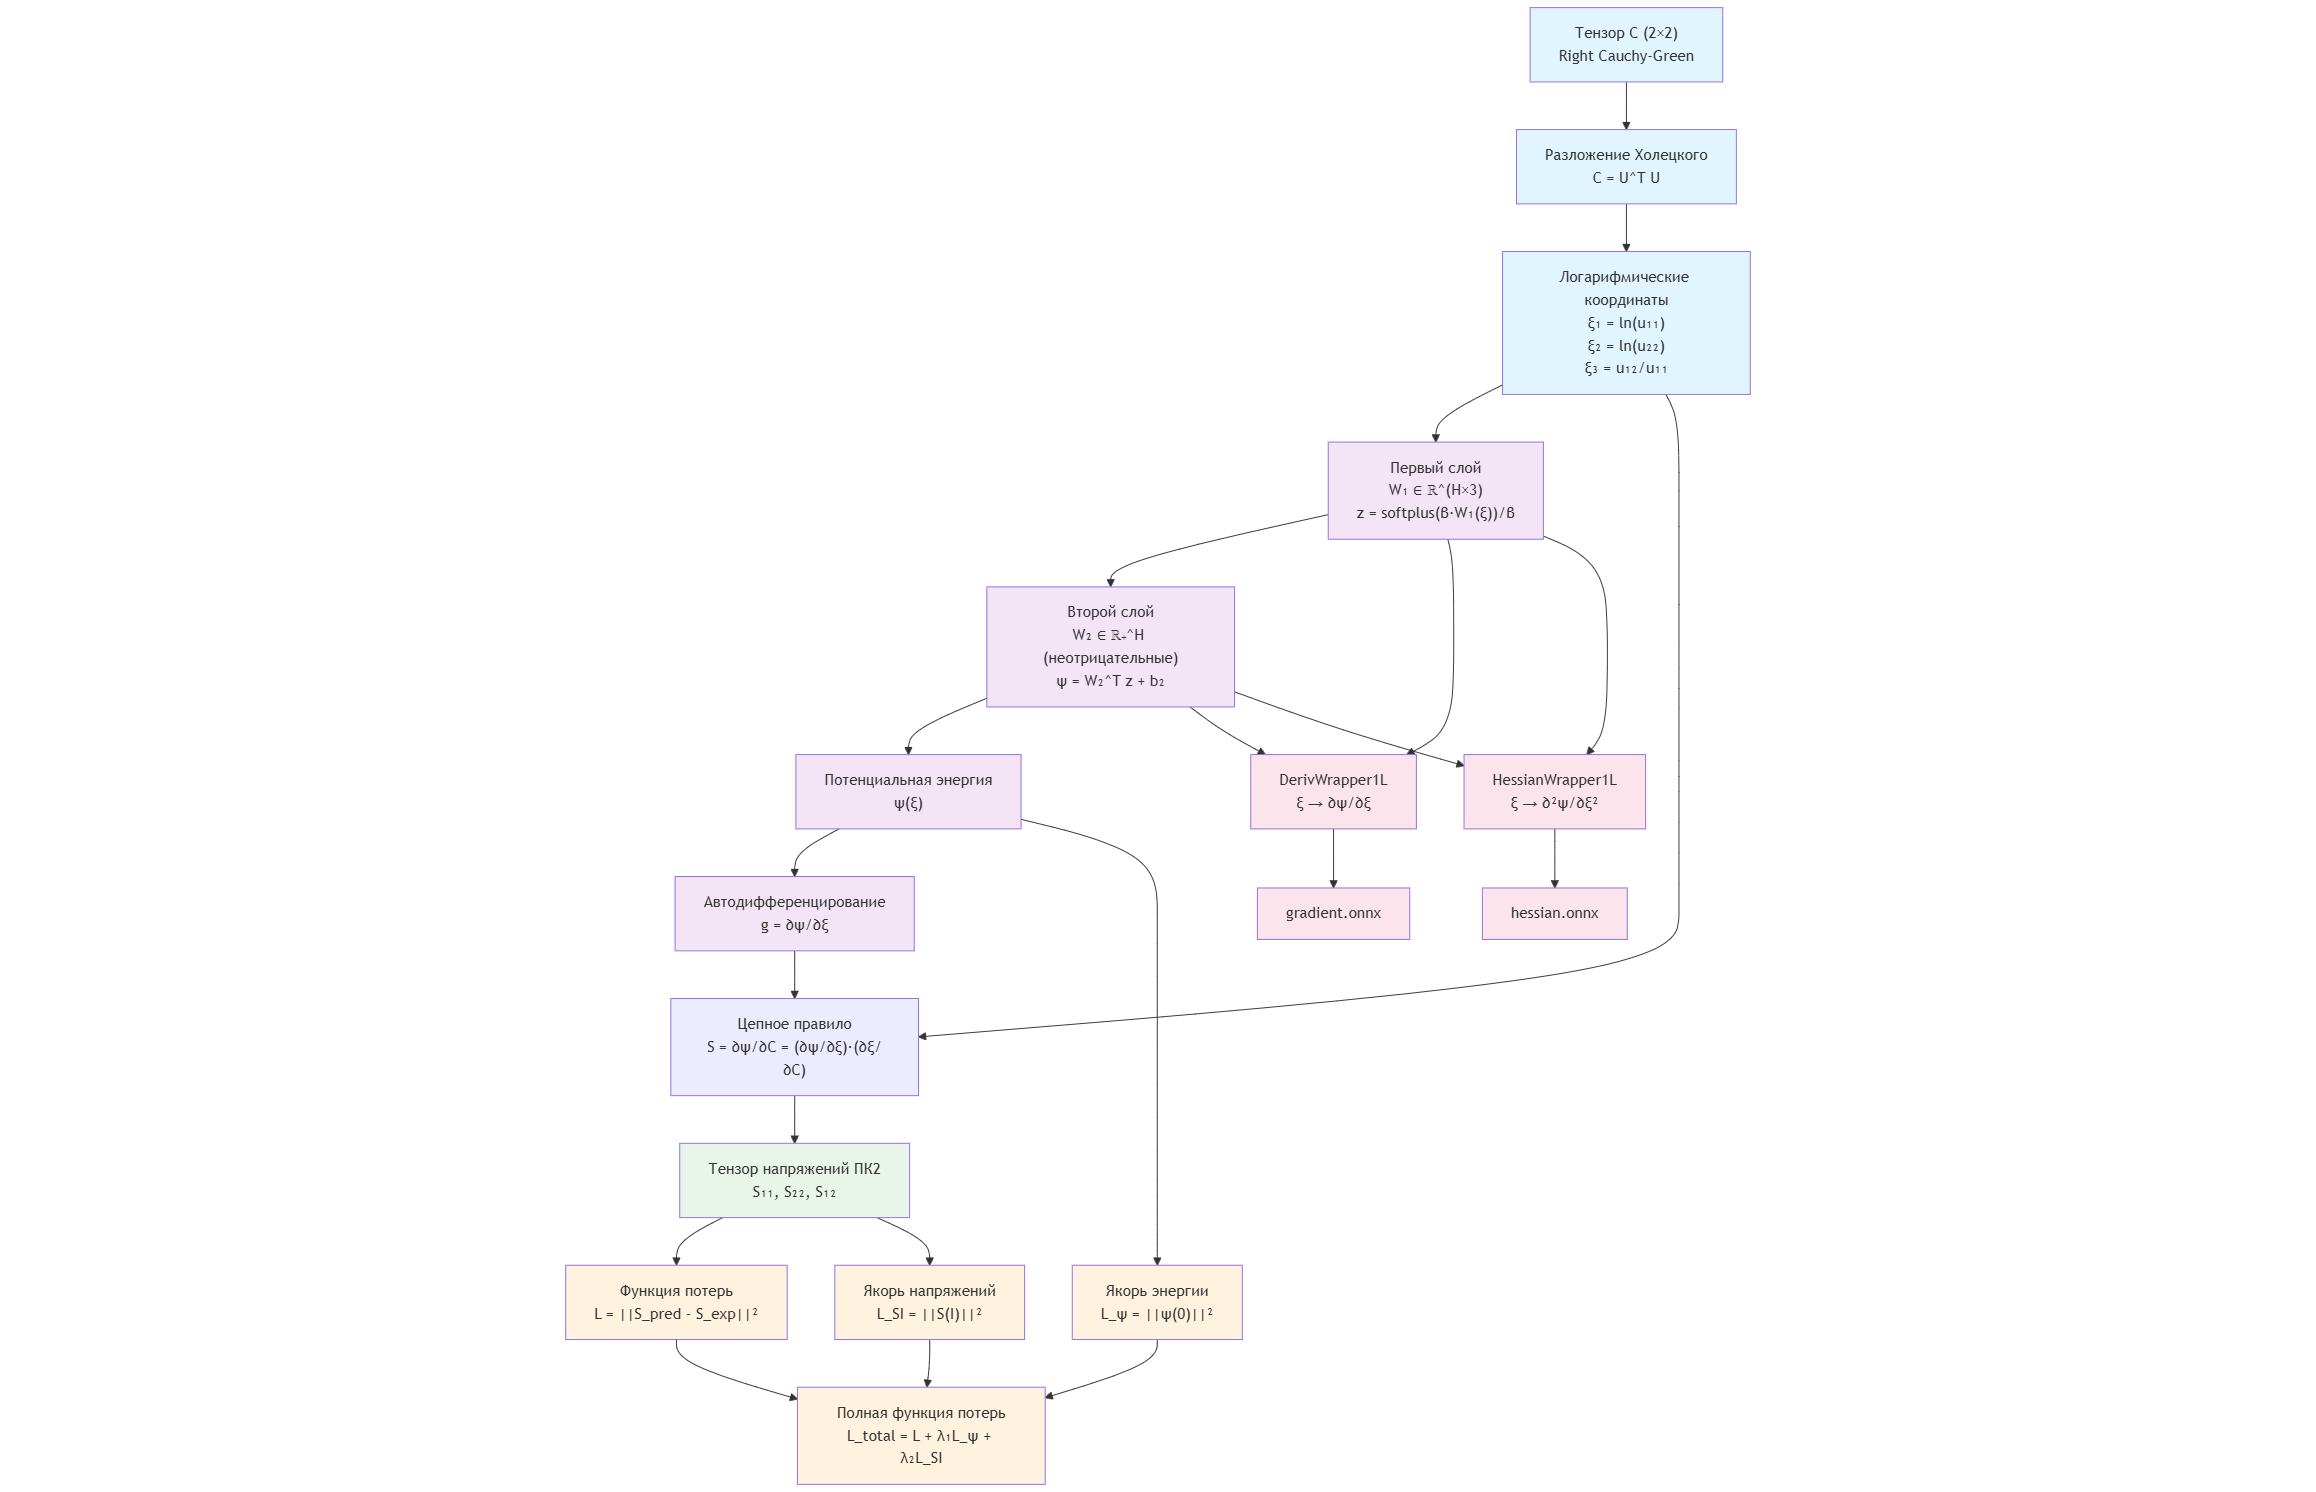
\includegraphics[width=1.3\textwidth]{img/clann_arc.png}
\caption{Схема вычислительного процесса CLANN: от входного тензора до функции потерь. Показаны этапы обработки входных данных, вычисления нейросетью, дифференцирования и формирования функции потерь.}
\label{fig:clann_architecture}
\end{figure}

\textbf{Аналитические выражения для производных энергии}

\textbf{Градиент энергии деформации}

Аналитическое дифференцирование функции энергии по переменным \(\xi\) даёт выражение для градиента:

\begin{equation}
 \vect{r} = \nabla_\xi \psi_{\mathrm{phys}} = \vect W_1^T \left( \vect W_2 \odot \sigma(\beta (\vect W_1 \vect \xi + \vect b_1)) \right) - \vect r_0,
\label{eq:energy_gradient}
\end{equation}
где $\sigma(x) = \frac{1}{1 + e^{-x}}$ - сигмоида, 
а операция $\odot$ обозначает поэлементное произведение (Hadamard product). 
Данное выражение демонстрирует, что градиент энергии является линейной комбинацией строк матрицы $\vect W_1^T$ с весами, 
определяемыми произведением выходных весов $\vect W_2$ и значений функции активации $\sigma(\beta (\vect W_1 \vect\xi + \vect b_1))$.

\textbf{Гессиан энергии деформации}

Вторые производные энергии по переменным \(\xi\) определяют гессиан, который имеет следующую аналитическую форму:

\begin{equation}
 H_{ij} = \sum_h \sigma'_h\,W_{2,h}\,W_{h,i}W_{h,j},
\label{eq:energy_hessian}
\end{equation}

где $\sigma' = \beta\,\sigma(1-\sigma)$ - производная сигмоиды, 
$\sigma=\operatorname{sigmoid}(\beta s)$, а $s=\vect W_1\xi+\vect b_1$.

\textbf{Материальная устойчивость и положительная определённость}

% Строгая выпуклость функции энергии \(\psi(\xi)\) по переменным \(\xi\)
% имеет фундаментальное значение для материальной устойчивости гиперупругого материала. 
% Как показано в классических работах Болла (Ball, 1977) и Чиарлета (Ciarlet, 1988), 
% выпуклость энергии деформации является необходимым и достаточным условием для существования и единственности решения 
% задачи равновесия в нелинейной теории упругости.

Из строгой выпуклости \(\psi(\xi)\) следует положительная определённость гессиана:
\begin{equation}
 \vect H = \frac{\partial^2\psi}{\partial\xi^2} > 0,
\label{eq:positive_hessian}
\end{equation}

что обеспечивает положительную определённость касательных модулей упругости 
$\mathbb{C} = \partial^2\psi/\partial\vect C^2$ через цепное правило дифференцирования. 
Это свойство важно для численной стабильности конечно-элементных расчётов, 
поскольку на практике обеспечивает сходимость метода Ньютонаи отсутствие сингулярностей в матрице жёсткости.

% \textbf{Физическая интерпретация гессиана}

% Гессиан $H_{ij}$ представляет собой матрицу касательных модулей упругости в логарифмических координатах Лапласа. Положительная определённость этой матрицы, обеспечиваемая архитектурой ICNN, гарантирует материальную устойчивость в том смысле, что любое малое возмущение деформации приводит к увеличению энергии деформации. Это свойство является фундаментальным для гиперупругих материалов и соответствует принципу Ле Шателье-Брауна в термодинамике.

% Структура выражения \eqref{eq:energy_hessian} отражает аддитивный вклад каждого скрытого нейрона в общую жёсткость материала, что обеспечивает физически интерпретируемую параметризацию механических свойств.

% \subsection{Функция потерь и процесс обучения: физические ограничения и регуляризация}

% \textbf{Основная функция потерь: минимизация невязки напряжений}

В рамках предложенного подхода обучение модели осуществляется путём минимизации функции потерь, 
которая количественно характеризует невязку между предсказанными и экспериментальными значениями напряжений:

\begin{equation}
 L = \frac{1}{N}\sum_{i=1}^N \lVert \vect S^{(i)}_{\text{pred}} - \vect S^{(i)}_{\text{exp}} \rVert^2.
\label{eq:main_loss_function}
\end{equation}

Для минимизации функции потерь \eqref{eq:main_loss_function} используется оптимизатор Adam \cite{kingma2014adam}, 
который широко используется в задачах машинного обучения. 
Процесс оптимизации включает вычисление градиентов по всем параметрам сети и обновление весов 
с использованием адаптивных моментов первого и второго порядка.

Такое построение архитектуры CLaNN обеспечивает выполнение всех необходимых физических свойств гиперупругой модели: 
\textbf{термодинамическая корректность} достигается через строгое соблюдение соотношения \eqref{eq:chain-rule}, 
что гарантирует консервативность напряжений $\oint \vect{S}:\mathrm{d}\vect{C} = 0$ и согласованность с законами 
термодинамики; 
\textbf{материальная устойчивость} обеспечивается и существенно улучшается за счёт строгой выпуклости функции энергии 
$\psi(\boldsymbol{\xi})$, гарантируемой архитектурой ICNN ($\vect{W}_2 \ge 0$, выпуклая неубывающая активация); 
\textbf{объективность} автоматически выполняется благодаря параметризации через тензор 
Коши-Грина $\vect{C} = \vect{F}^{\top}\vect{F}$, обеспечивая инвариантность относительно поворотов и симметрию напряжений; 
\textbf{строгая неотрицательность и коэрцитивность энергии} обеспечиваются архитектурной калибровкой 
$\psi_{\mathrm{phys}}(\boldsymbol{\xi}) = \mathbf{W}_2^{\top}(z - z_0) - \mathbf{r}_0^{\top}\boldsymbol{\xi} + \tfrac{\gamma}{2}\|\boldsymbol{\xi}\|^2$ 
с $\gamma>0$, что даёт $\psi_{\mathrm{phys}}(\mathbf{0})=0$, $\psi_{\mathrm{phys}}(\boldsymbol{\xi})>0$ при $\boldsymbol{\xi}\ne\mathbf{0}$ и 
$\psi_{\mathrm{phys}}(\boldsymbol{\xi})\to\infty$ при $\|\boldsymbol{\xi}\|\to\infty$ (см. clann\_math.markdown, § Потенциал); 
% \textbf{численная стабильность} достигается через логарифмическую параметризацию Лапласа \eqref{eq:laplace_coords}, которая корректно обрабатывает большие деформации и предотвращает нефизичные значения; 
наконец, \textbf{физические ограничения} \eqref{eq:energy_constraints} обеспечиваются архитектурой сети CLaNN: монотонные, выпуклые функции активации,
неотрицательные весовые коэффициенты, центрирование энергии деформации $\psi$ и отклика $\vect r$.



\section{Виртуальный эксперимент}

Мы используем синтетические экспериментальные данные для тестирования CLaNN 
на изотропном надуваним однородной и неоднородной по толщине мембраны. 
А именно, мы генерируем данные с помощью виртуальных экспериментов на плоских растяжениях образца и используем их в качестве входных данных для 
обучения CLaNN, без какого-либо дополнительного знания об изотропности/анизотропии образца и форме потенциала.
 
Обучение модели проводилось на численных экспериментальных данных, 
полученных при двухосном растяжении образца с геометрией мальтийского креста (Рисунок \ref{fig:malt_geometry}).
С неогуковской гиперупругой моделью для двумерной мембраны \cite{ogden1997nonlinear}
% \begin{equation}
%  \Psi(\vect C, T) = h_0\, \frac{\mu}{2}\,\big(\operatorname{tr}\vect C + T^2 - 3\big),
% \label{eq:neo_hookean_energy}
% \end{equation}
% где $\vect C$ — двумерный правый тензор деформаций Коши–Грина (вдоль срединной поверхности), $T$ — растяжение по толщине (параметр мембранного приближения), $h_0$ — начальная толщина мембраны, а $\mu = 0.432 \,\text{МПа}$ — модуль сдвига. Для несжимаемого материала выполняется связь $\sqrt{\det \vect C}\,T = 1$.

Причем данные для обучения собирались из одного центрального элемента сетки, что соответствует ограничениям эквивалетного 
натурного эксперимента, в котором невозможно установить без предположения модели материала полное поле напряжения в образце.

Для решения задачи равновесия гиперупругой мембраны используется метод описанный в \cite{ddaniso2024}.

\begin{figure}[H]
  \centering
  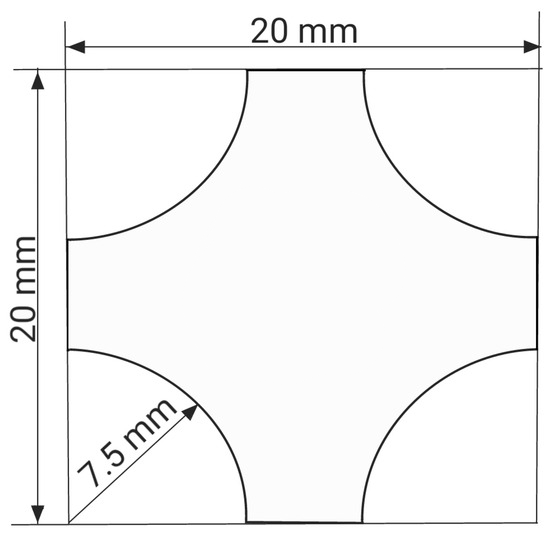
\includegraphics[width=0.5\textwidth]{img/malt_geom.png}
  \caption{Размеры образца биоматериала в форме мальтийского креста. 
  Радиус вырезов одинаков для всех вырезов}
  \label{fig:malt_geometry}
\end{figure}

Схематическое представление протоколов показано на рисунке \ref{fig:malt_displacements}, где $w_i \in [0,1]$, $i \in \{1,4\}$
представляет собой долю от заданного максимального смещения $u_{\max}$ для $i$-го плеча: $w_i = 0$ 
соответствует неподвижному плечу, а $w_i = 1$ — соответствует плечу, чьё положение было сдвинуто и фиксировано на расстояние $u_{max}$. 
Изменяя $w_i$, можно получить различные типы экспериментов. 
В наших виртуальных экспериментах мы постепенно 
прикладываем смещение с определенным шагом $\Delta s$ до достижения максимального смещения. 
Смещение $w_i \cdot n \cdot \Delta s$ прикладывается к $i$-му плечу на $n$-м шаге, где $n = 1, \ldots, N$, 
$N = u_{\max}/\Delta s$ — количество шагов. 
Треугольная сетка для образца является квазиравномерной с размером ячейки $h_{\text{fit}} = 0.25$ мм, максимальное смещение 
$u_{\max} = 2$ мм и $\Delta s = 0.2$ мм. 
На каждом шаге мы собираем данные $(\vect C, \vect S)$ для всех треугольников, принадлежащих выбранной области наблюдения. 
Поскольку мы используем линейные ($P_1$) конечные элементы, значения $(\vect C, \vect S)$ постоянны на каждом треугольнике.

 \begin{figure}[H]
  \centering
  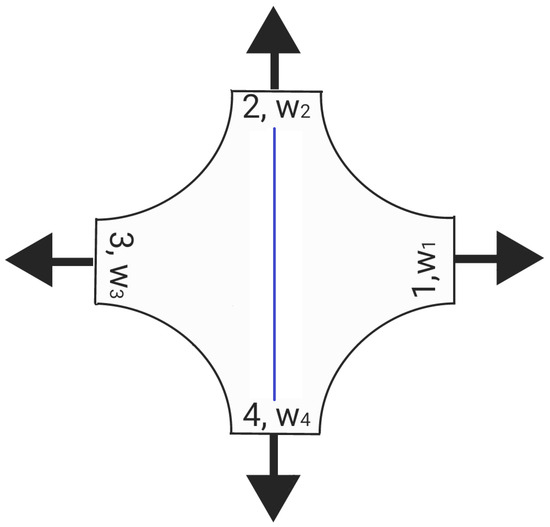
\includegraphics[width=0.5\textwidth]{img/malt_dirichlet.png}
  \caption{Схематическое представление протоколов. 
  Радиус вырезов одинаков для всех вырезов}
  \label{fig:malt_displacements}
\end{figure}
 
Наш предлагаемый тестовый протокол предполагает девять экспериментов:

\begin{table}[H]
\centering
\caption{Протоколы тестовых экспериментов}
\label{tab:test_protocols}
\begin{tabular}{|c|c|c|c|c|}
\hline
\textbf{№} & $w_1$ & $w_2$ & $w_3$ & $w_4$ \\
\hline
1 & 1 & 1 & 1 & 1 \\
2 & 1 & 0.75 & 1 & 0.75 \\
3 & 0.75 & 1 & 0.75 & 1 \\
4 & 1 & 0.5 & 1 & 0.5 \\
5 & 0.5 & 1 & 0.5 & 1 \\
6 & 1 & 1/3 & 1 & 1/3 \\
7 & 1/3 & 1 & 1/3 & 1 \\
8 & 1 & 0 & 1& 0 \\
9 & 0 & 1 & 0 & 1 \\
\hline
\end{tabular}
\end{table}

\subsubsection{Правила отбора данных}
\paragraph{Центральное окно $w$.}
Окно задаётся в исходной конфигурации $\Omega_0$ как центральная область вокруг геометрического центра образца, согласованная с осями расчётной сетки.
Для $w=\text{1-элемент}$ берётся единственный центральный треугольник (ячейка, чей барицентр ближайший к центру $\Omega_0$).
Для $w=5\times5$ мм и $w=10\times10$ мм берётся квадрат со сторонами 5 и 10 мм соответственно, центрированный в центре образца; для $w=\text{всё поле}$ — вся область $\Omega_0$.
Наблюдения включают все треугольники, барицентры которых $\mathbf{X}_T$ лежат внутри выбранного окна $\mathcal{W}_w\subset\Omega_0$.
% TODO: добавить мощность окна в элементах сетки

\paragraph{Состав наблюдений (данные).}
На каждом шаге нагружения $n=1,\dots,N$ и для каждого треугольника $T\in\mathcal{T}_w$ (ячейки, попавшие в окно) фиксируется пара $(\vect C_T^{(n)},\,\vect S_T^{(n)})$, 
где $\vect C$ — правый тензор Коши–Грина, $\vect S$ — второй тензор Пиолы–Кирхгофа.
Единицы: размеры окна — мм; $\vect C$ — безразмерен; $\vect S$ — МПа.

\paragraph{Формирование выборок.}
Для фиксированных $(p,w)$ совокупность всех пар $(\vect C_T^{(n)},\,\vect S_T^{(n)})$ образует базовый набор $D(p,w)$, из которого формируются разбиения $D_{\mathrm{tr}}(p,w)$ и $D_{\mathrm{val}}(p,w)$.
Для заданных протокола $p$ (см. табл.~\ref{tab:test_protocols}) 
и окна центральной области образца 
$w\in\{\text{1-элемент},\,5\times5 мм,\,10\times10 мм,\,\text{всё поле}\}$ обозначим
\[
  D_{\mathrm{tr}}\equiv D_{\mathrm{tr}}(p,w),\qquad D_{\mathrm{val}}\equiv D_{\mathrm{val}}(p,w),
\]
где $D_{\mathrm{tr}}$ — обучающая, $D_{\mathrm{val}}$ — валидационная выборки.


Например, |D(\{1..10\}, \text{1-элемент})|= 90 точек данных правого тензора деформаций Коши-Грина $\vect C$ 
и второго тензора напряжений Пиолы-Кирхгофа $\vect S$ (Рисунок \ref{fig:training_data}).

\begin{figure}[H]
  \centering
  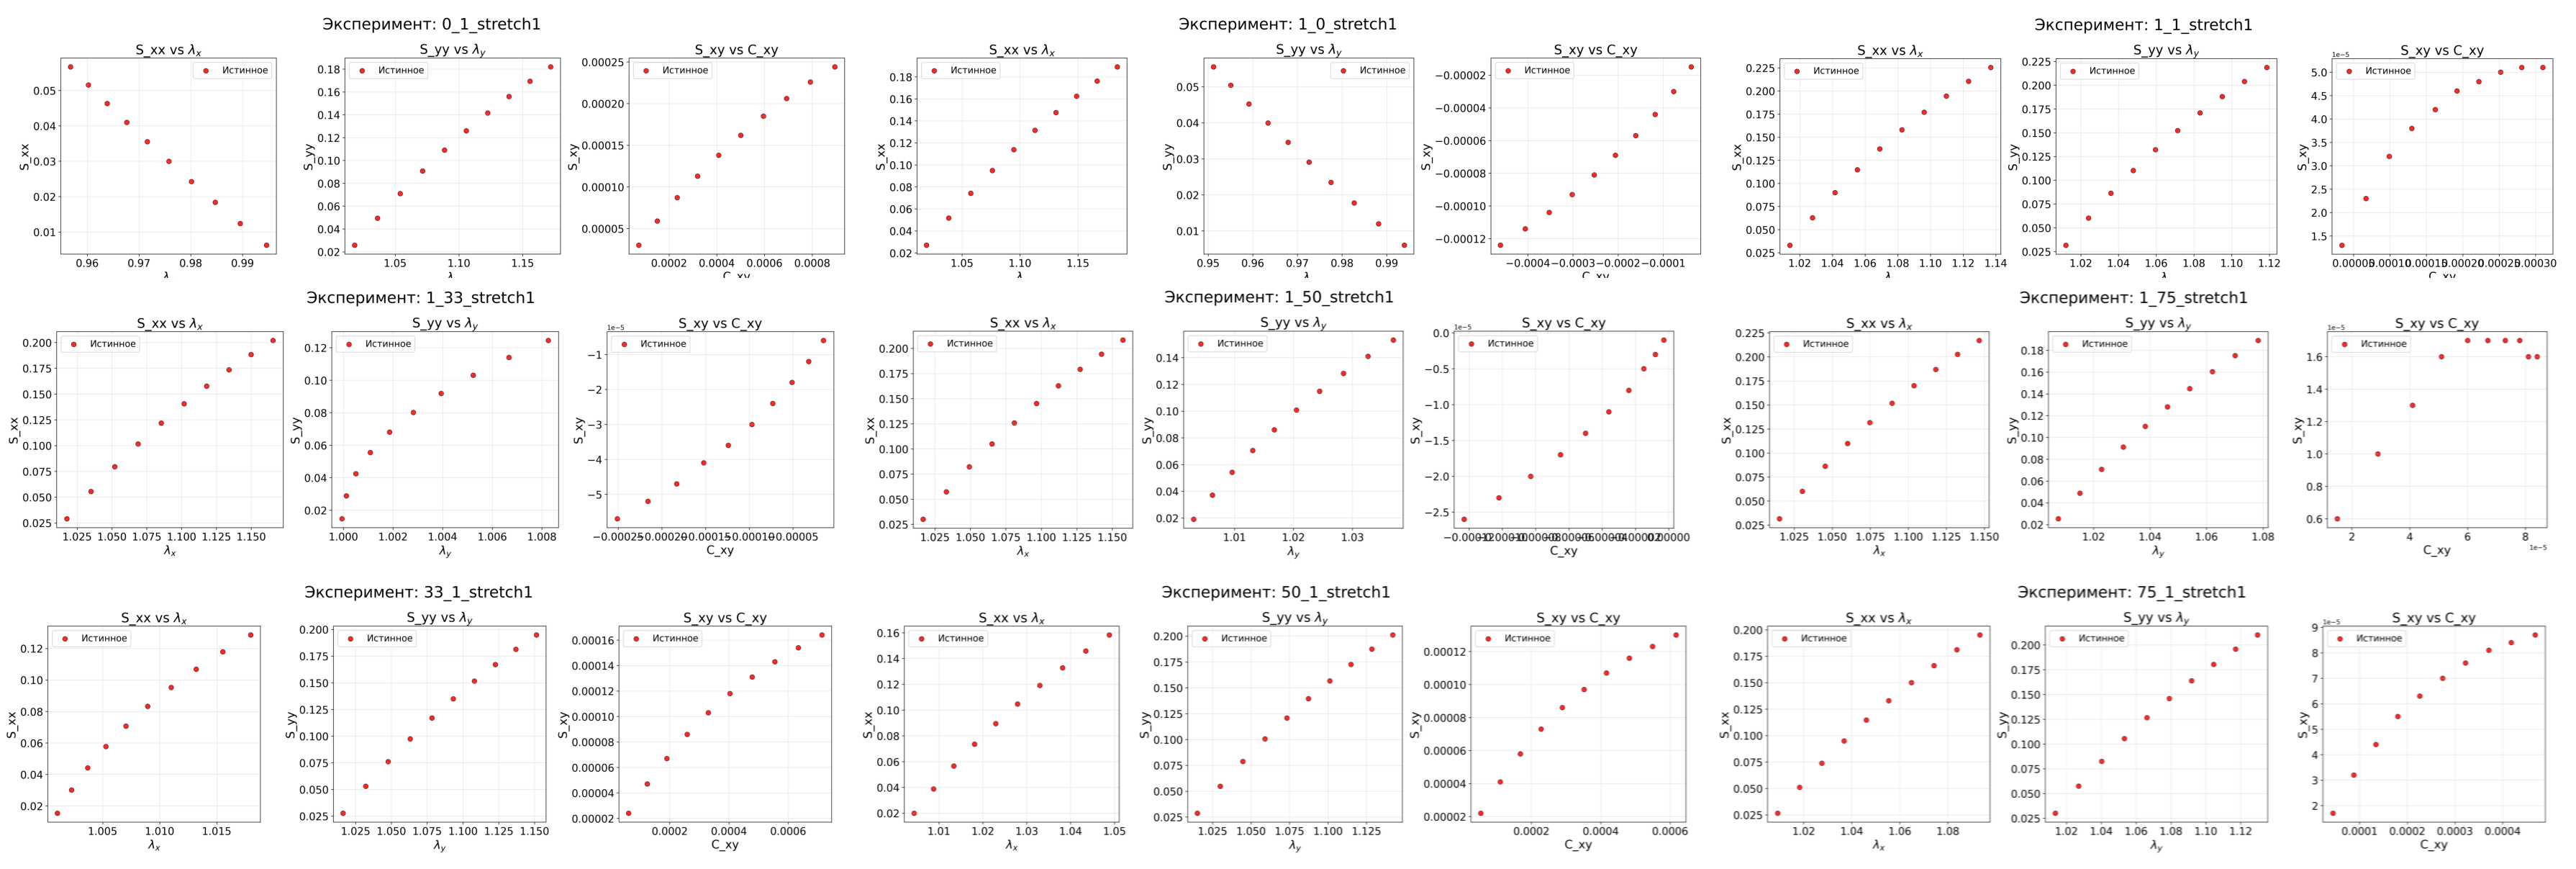
\includegraphics[width=1.0\textwidth]{img/all_stress_plots.png}
  \caption{Обучающий набор данных}
  \label{fig:training_data}
\end{figure}

Так как мы собираем данные из одного центрального элемента сетки, то растягивающие компоненты $xx, yy$ тензоров деформации $\vect C$ и напряжения
$\vect S$ имеют значения на 2-3 порядка большие чем сдвиговые компоненты $xy$.

\textbf{Гиперпараметры оптимизации:}
\begin{itemize}
  \item Скорость обучения (learning rate): $0.001$
  \item Размер батча (batch size): $4$ при обучении на 90 точек данных и $128$ для остальных обучающих наборов данных.
  % \item Веса физических ограничений: $\lambda_{\text{SI}} = 0.1$, $\lambda_{\psi} = 0.1$
  \item Архитектура: 16 нейронов на скрытом слое
  \item Сглаживающий параметр $\beta$: $10$
\end{itemize}

\textbf{Результаты обучения:}
Процесс оптимизации показал высокую эффективность: ошибка аппроксимации снизилась на 5 порядков за менее чем 5000 эпох (рисунок \ref{fig:loss_curve}), 
что демонстрирует как качество предложенной архитектуры, так и корректность выбора гиперпараметров. 
Столь быстрая сходимость обусловлена строгой выпуклостью функции энергии, что обеспечивает единственность 
минимума и отсутствие локальных минимумов в пространстве параметров.

\begin{figure}[H]
  \centering
  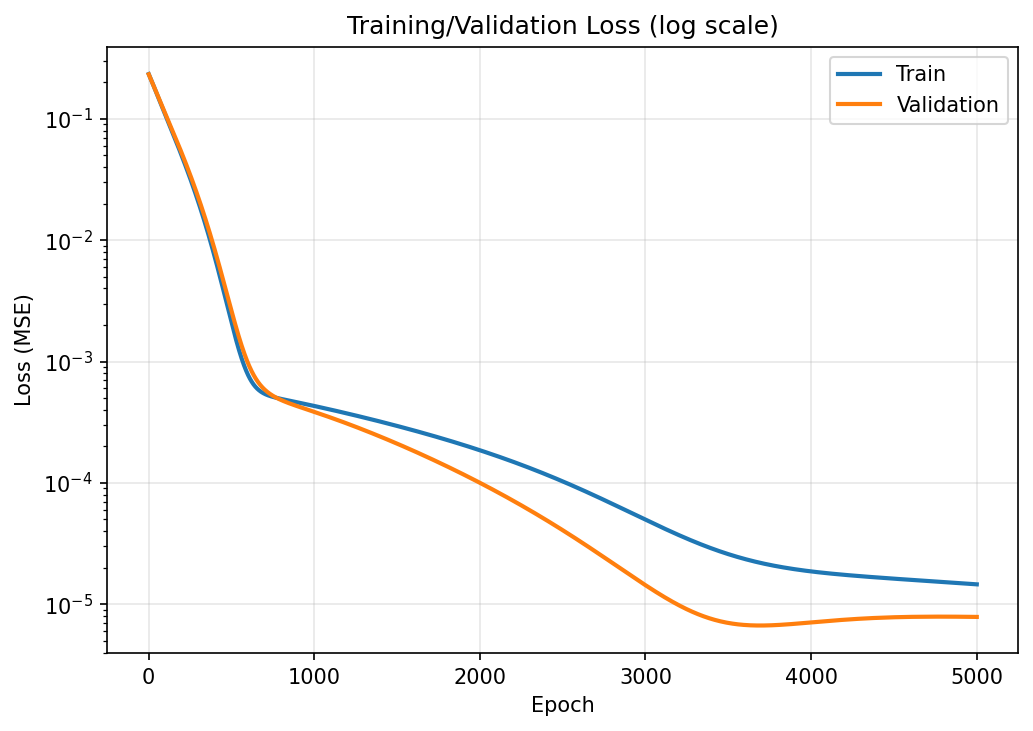
\includegraphics[width=0.7\textwidth]{img/loss_curve.png}
  \caption{Кривая функции потерь при обучении на 90 точках данных}
  \label{fig:loss_curve}
\end{figure}


\subsection{Интерполяция и экстраполяция кривых нагружения}
  Сначала мы проверили, как модель CLaNN интерполирует и экстраполирует кривые нагружения, используя выборки
  $D_{\mathrm{tr}}(p,w)$ и $D_{\mathrm{val}}(p,w)$ для заданного окна наблюдения $w$.
  Для оценки качества использовали коэффициент детерминации $R^2$:
  \begin{equation}
  R^2 = 1 - \frac{\sum_{i=1}^n (y_i - \hat{y}_i)^2}{\sum_{i=1}^n (y_i - \bar{y})^2},
  \label{eq:r_squared}
  \end{equation}
  где $y_i$ — экспериментальные значения, $\hat{y}_i$ — предсказания модели, $\bar{y}$ — среднее экспериментальных значений, $n$ — количество точек данных.
  Метрику качества фиксируем как коэффициент детерминации (см. \eqref{eq:r_squared}):
\[
  R^2_{\alpha}(D_{\mathrm{val}}),\qquad \alpha\in\{xx,yy,xy\}.
\]

  \textbf{Интерполяция.}  

  Для тестирования спосбности архитектуры CLaNN мы использовали данные из 
  10 точек кривой нагружения равнодвухосного растяжения мембраны $p=1$, 
  окно наблюдения $w=\text{1-элемент}$:
  
  $D_{in} = D(p{=}1,\,w{=}\text{1-элемент}),\, n = 1..10,$
  
  $D_{\mathrm{tr}}=\{\forall (\vect {C}^{n_{tr}}, \vect{S}^{n_{tr}}) \in D_{in}|\; n_{tr}=\{1,5,10\}\},$
  
  $D_{\mathrm{val}}=\{\forall (\vect {C}^{n_{val}}, \vect{S}^{n_{val}}) \in D_{in}|\; n_{val}=n \backslash  n_{tr}\}.$

  CLaNN показал высокую точность интерполяции кривой нагружения равнодвухосного растяжения мембраны 
  для растягивающих компонент $R^2_{xx}=0.999$, $R^2_{yy}=0.999$, и отсуствие достоверного предсказания сдвиговых 
  компонент $R^2_{xy}=0$ (рисунок \ref{fig:interpolation}).
  
  \begin{figure}[H]
    \centering
    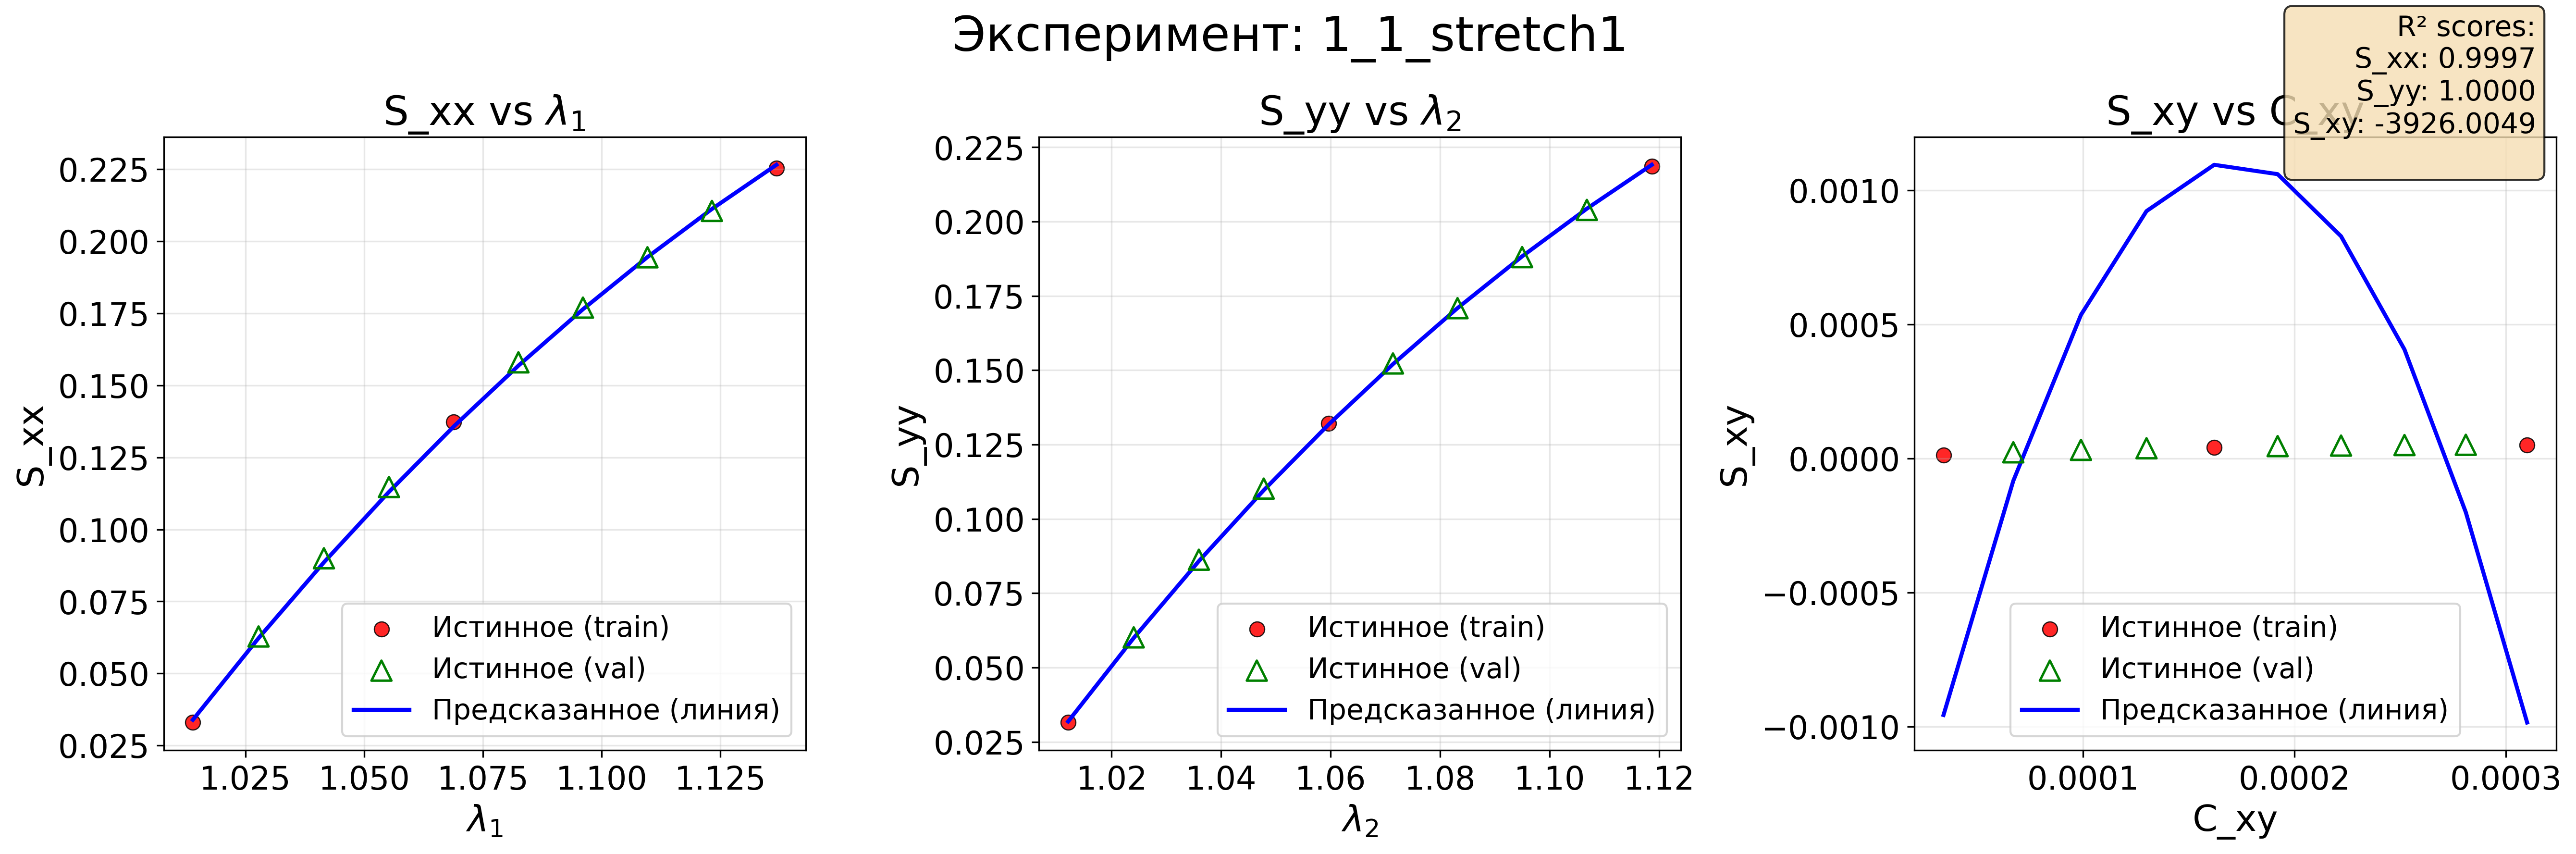
\includegraphics[width=1.0\textwidth]{img/interpolation.png}
    \caption{Кривая нагружения для равнодвухосного растяжения}
    \label{fig:interpolation}
  \end{figure}
  
  \textbf{Экстраполяция.}
  
  Для проверки способности к экстраполяции использовали обучение на равнодвухосном растяжении (протокол 1) и валидацию на неравнодвухосном (протокол 9), 
  окно наблюдения $w=\text{1-элемент}$:
  
  $D_{\mathrm{tr,in}} = D(p{=}1,\,w{=}\text{1-элемент}),\, n = 1..10,$
  
  $D_{\mathrm{val,in}} = D(p{=}9,\,w{=}\text{1-элемент}),\, n = 1..10,$
  
  CLaNN показал высокую точность экстраполяции для растягивающих компонент $R^2_{xx}=0.993$, $R^2_{yy}=1.0$, и отсутствие достоверного предсказания сдвиговой компоненты $R^2_{xy}=0$ (рисунок \ref{fig:extrapolation}).


  \begin{figure}[H]
    \centering
    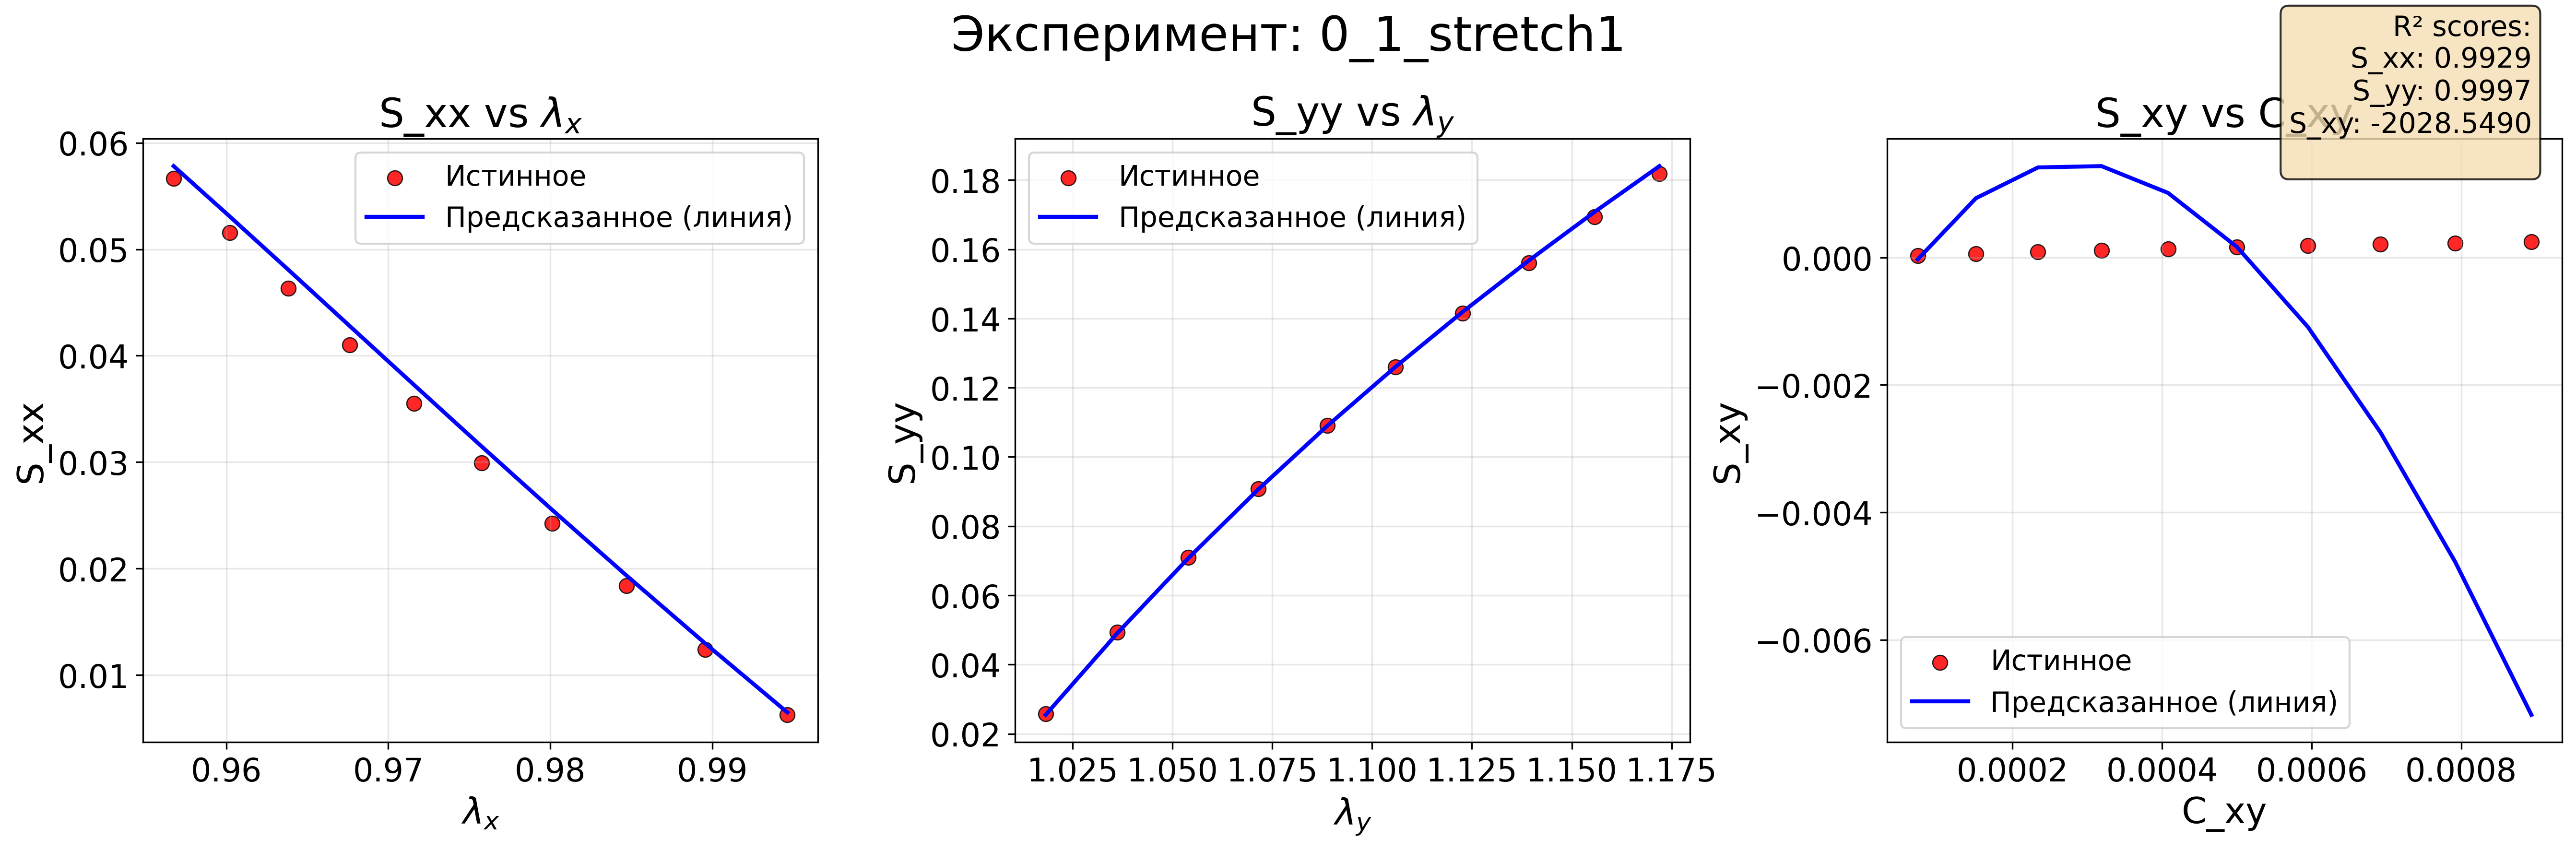
\includegraphics[width=1.0\textwidth]{img/extrapolation.png}
    \caption{Кривая нагружения для неравнодвухосного растяжения}
    \label{fig:extrapolation}
  \end{figure}
   
  Таким образом, CLaNN способен интерполировать и экстраполировать кривые нагружения с высокой точностью, что свидетельствует о его способности к обобщению на новые данные.
  Однако, не справляется с предсказанием сдвиговых компонент $\vect S_{xy}$, что может быть связано с тем, что данные для сдвиговых компонент не достаточно большие.
  
\subsection{Раздутие мембраны}

  Для проверки способности CLaNN, мы поставили численный эксперимент по раздутию круглой мембраны радиусом 25 мм.
  Мембрана закреплена по внешнему контуру и подвергается равномерному растяжению по всей поверхности при заданном давлении
  5 МПа. 
  Как референс мы использовали результаты численного эксперимента с использованием гиперупругой модели Нео-Гука с тем же параметром сдвига, 
  что и при генерации данных для обучения CLaNN.
  
  Мы использовали два поля толщин элементов $T$: 1) с гомогенным полем толищны 0.54 мм. 
  2) с гетерогенным полем толищны, где в в окружности высекается два пораболических сектора с толщиной 2 мм
  и остальной части мембраны 0.54 мм (Рисунок \ref{fig:membrane_thickness}). 

  В качестве метрики ошибки мы использовали относительную ошибку между предсказанными и эталонными значениями напряжений:
  \begin{equation}
    \epsilon = \frac{\| \vect S - \vect S_{\text{ref}} \|}{\| \vect S_{\text{ref}} \|},
  \end{equation}
  где $\vect S$ — предсказанные значения напряжений, $\vect S_{\text{ref}}$ — эталонные значения напряжений.

  А также для сравнения сдвиговых компонент напряжений использовали P1 относительную ошибку \cite{xie2024p1}, которая является комбинацией относительной и абсолютной ошибок и 
  более чувствительна к значениям близким к нулю:
  \begin{equation}
    \epsilon_{P1} = \frac{\| \vect S - \vect S_{\text{ref}} \|}{s_0 + \| \vect S_{\text{ref}} \|},
  \end{equation}
  где $\vect S$ — предсказанные значения напряжений, $\vect S_{\text{ref}}$ — эталонные значения напряжений, $s_0 = max(\vect S_{\text{pred}})$ — масштаб абсолютной толерантности (в единицах напряжения).

  \begin{figure}[H]
    \centering
    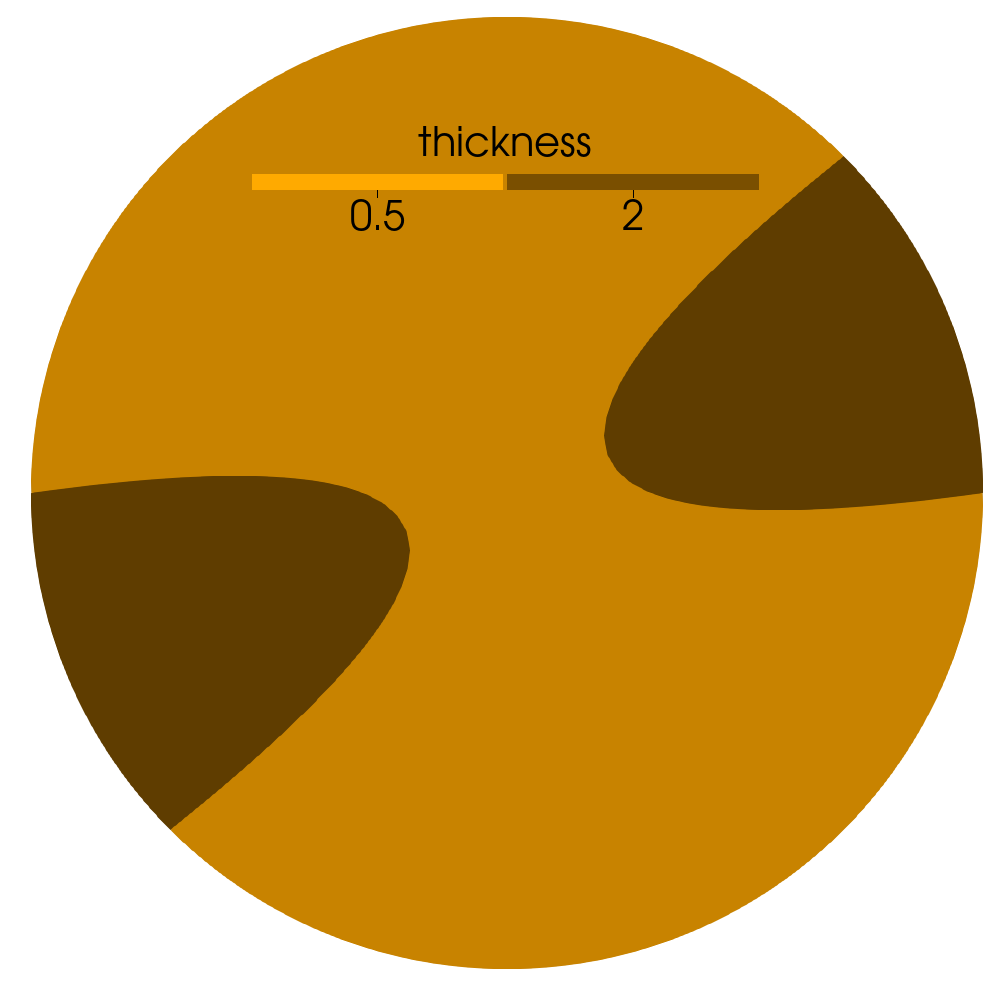
\includegraphics[width=0.25\linewidth]{img/het_circle.png}
    \caption{Гетерогенное поле толщин элементов $T$ круглой мембраны.}
    \label{fig:membrane_thickness}
  \end{figure}
  % \begin{wrapfigure}{r}{0.35\textwidth}
  %   \centering
  %   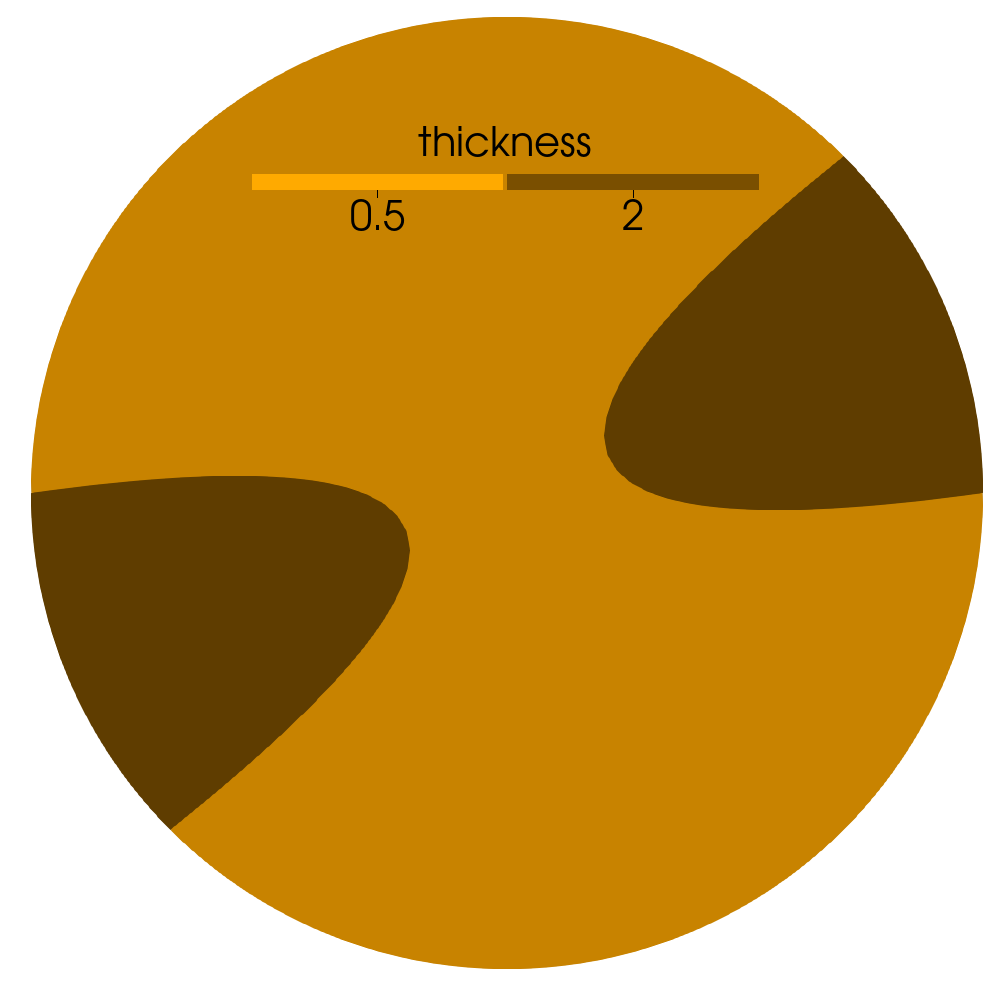
\includegraphics[width=\linewidth]{img/het_circle.png}
  %   \caption{Гетерогенное поле толщин элементов $T$ круглой мембраны.}
  %   \label{fig:membrane_thickness}
  % \end{wrapfigure}
  % Для геометрии с гетерогенным полем толщин референсные значения сдвиговой компоненты поля 2 тензора напряжений Пиолы-Кирхгофа 
  % $\vect S$ (Рисунок \ref{fig:numerical_experiment}) .

  \begin{figure}[H]
    \centering
    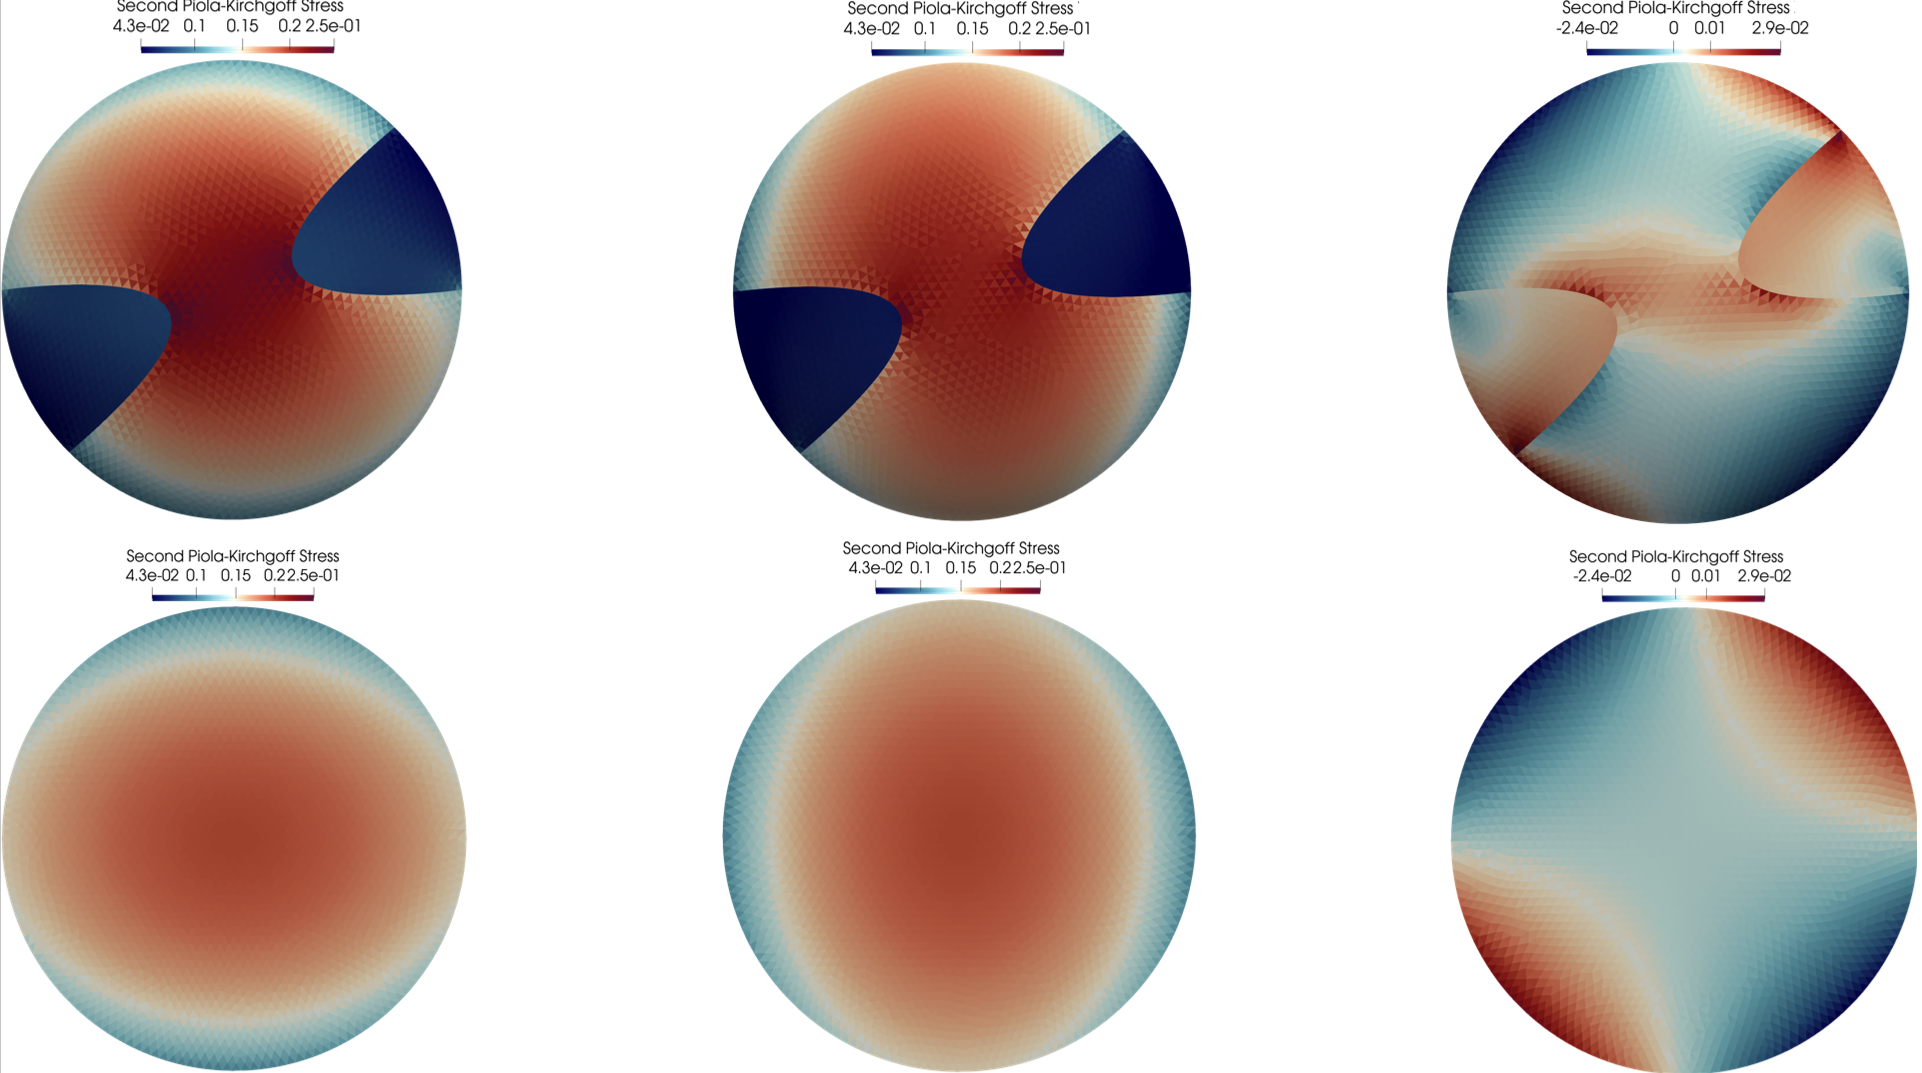
\includegraphics[width=1.0\textwidth]{img/Numerical/ref_stress.png}
    \caption{Поле напряжений $\vect S$ круглой мембраны с гетерогенным и гомогенным полем толщин элементов $T$.}
    \label{fig:numerical_experiment}
  \end{figure}
  
  В результате численного эксперимента на раздутие мембраны с гиперупругим определяющим соотношением CLaNN,
  используя набор данных $D (\{1..10\}, w=\text{1-элемент})$ для обучения, мы получили поле напряжений 2 тензора Пиолы-Кирхгофа 
  $\vect S$ для гомогенной и гетерогенной мембраны по толщине и сравнили его
  с референсными значениями (Рисунок \ref{fig:numerical_experiment}) и построили поле ошибок $\epsilon$ и $\epsilon_{P1}$ (Рисунок \ref{fig:numerical_errors}).
  Сдвиговая компонента напряжений $\vect S_{xy}$ показывает наибольшую ошибку для гетерогенной мембраны, 
  что может быть связано с тем, что данные для сдвиговых компонент не достаточно большие. Поэтому мы последовательно 
  расширяли набор данных для обучения до $D (\{1..10\}, w=\text{5x5})$, $D (\{1..10\}, w=\text{10x10})$, $D (\{1..10\}, w=\text{все поле})$, 
  и получили более точные результаты (Рисунок \ref{fig:numerical_errors}).

  \begin{figure}[H]
    \centering
    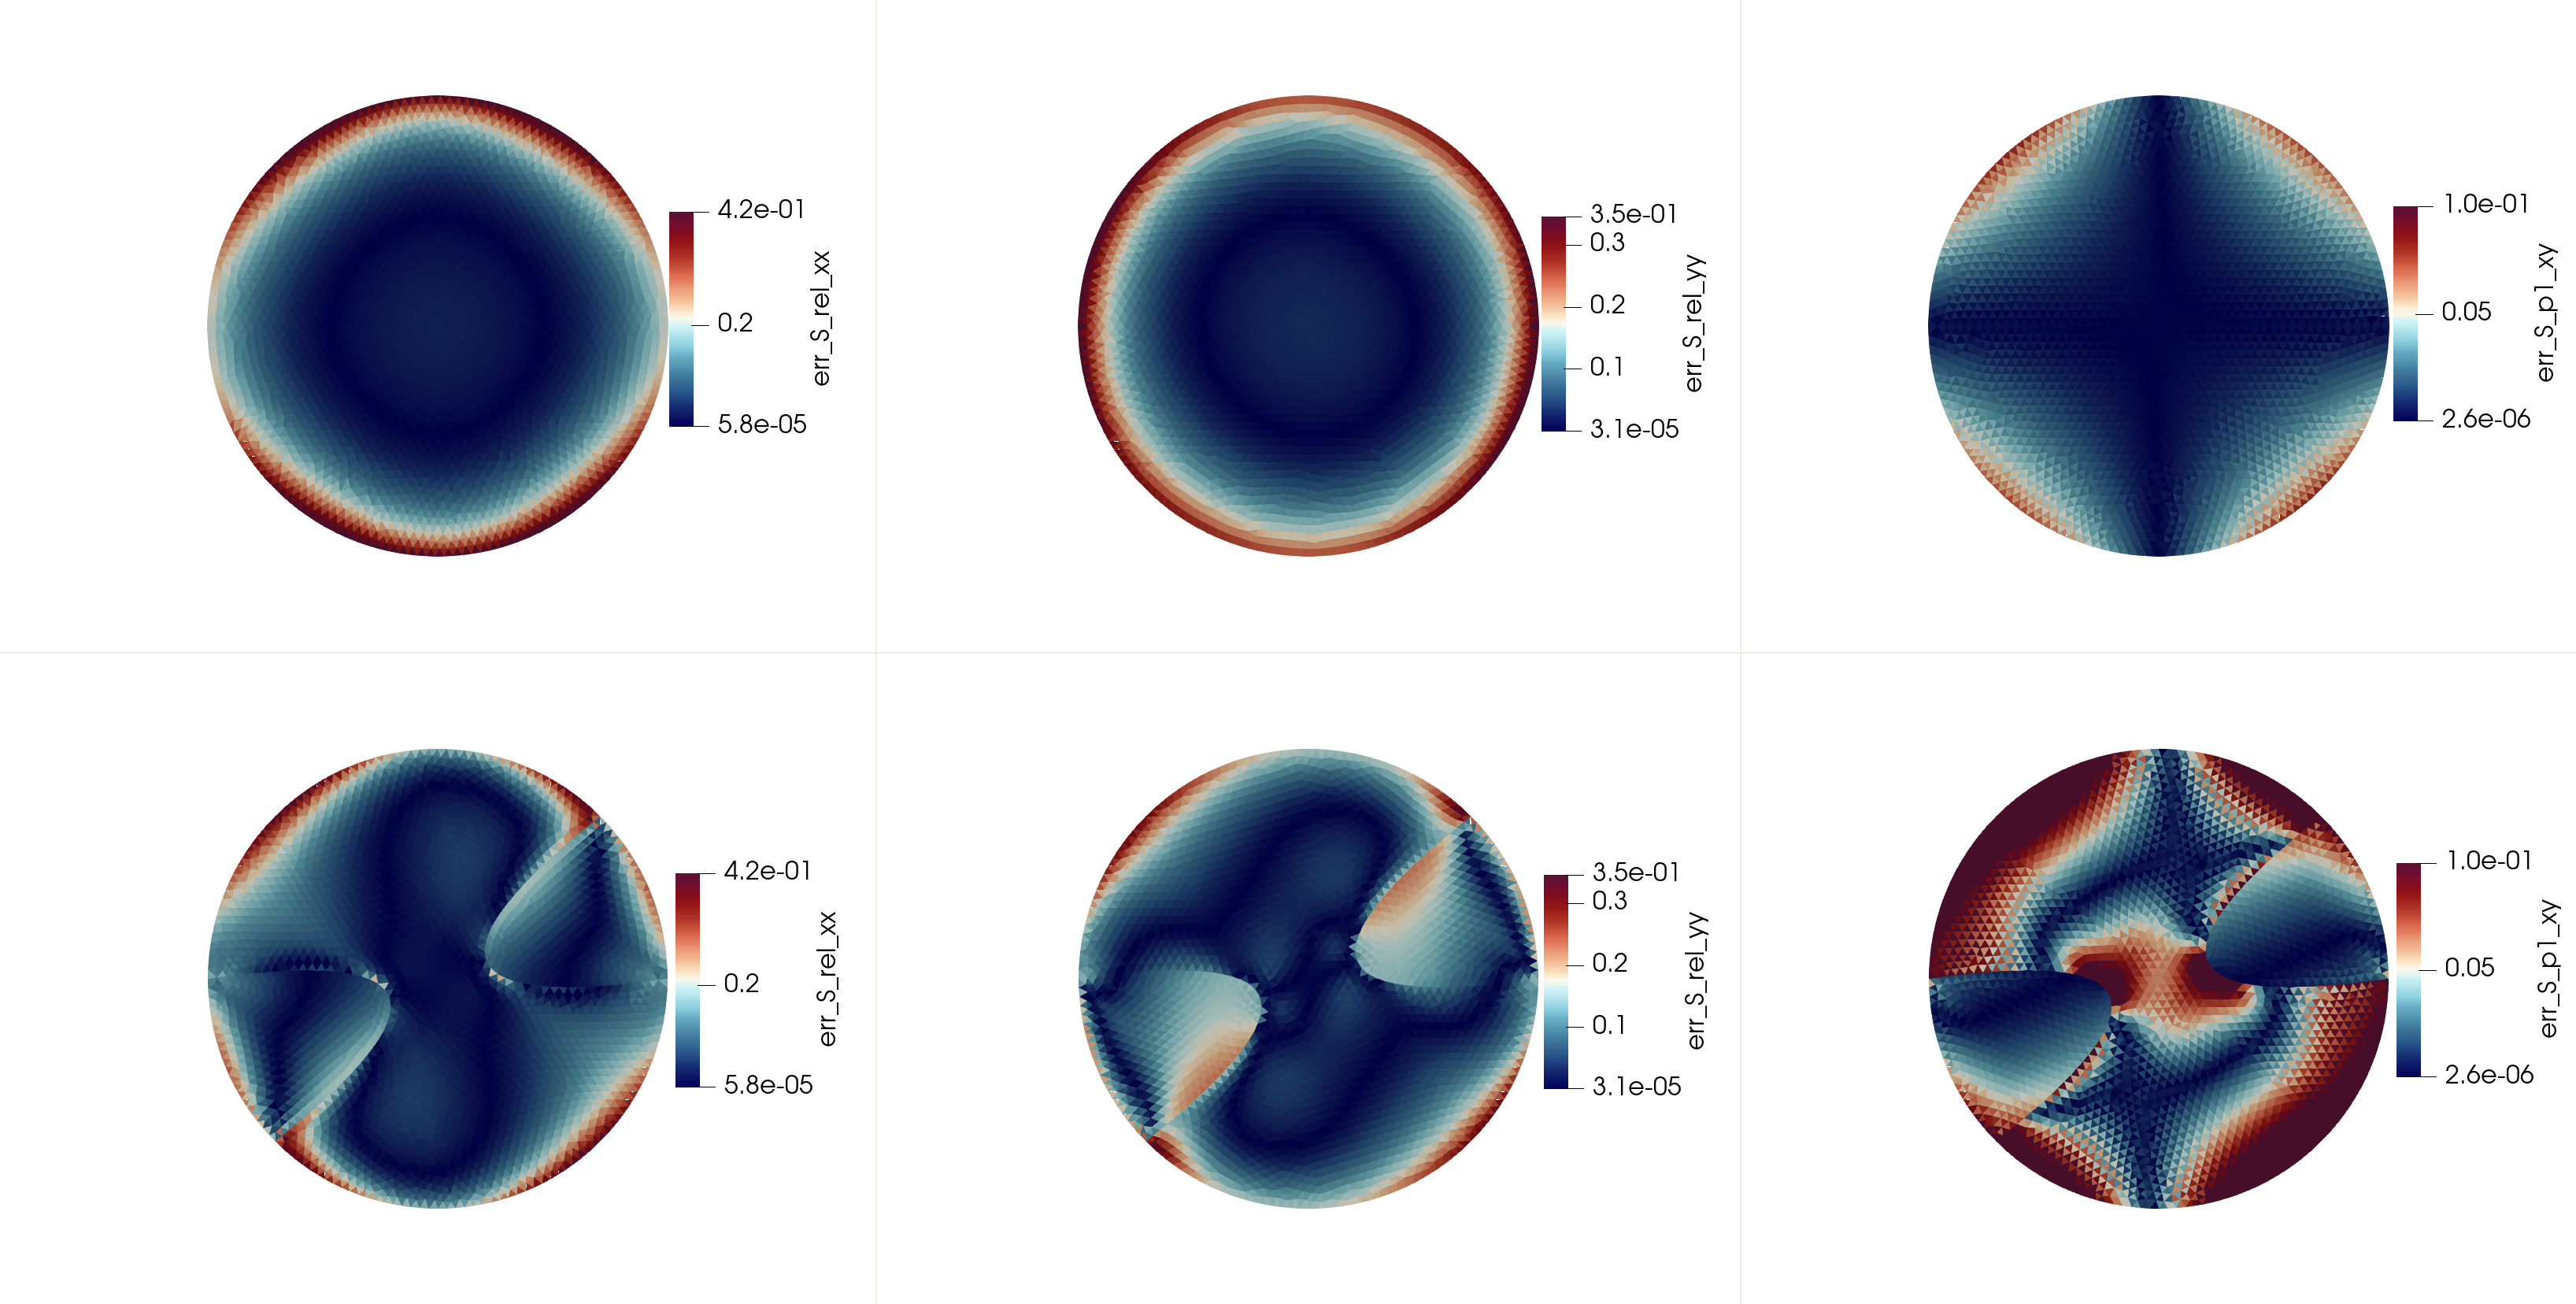
\includegraphics[width=0.7\textwidth]{img/Numerical/errs.png}
    \caption{Поле ошибок между предсказанными и эталонными значениями напряжений.}
    \label{fig:numerical_errors}
  \end{figure}
  


\begin{table}[htbp]
\centering
\caption{Сводка проведенных экспериментов по обучению и валидации модели CLANN}
\label{tab:experiments_summary}
\begin{tabular}{|p{2.3cm}|p{2.2cm}|p{2.2cm}|p{1.3cm}|p{2.3cm}|p{1.5cm}|p{2.5cm}|}
\hline
\multicolumn{4}{|c|}{\textbf{Обучение}} & \multicolumn{3}{c|}{\textbf{Валидация}} \\
\hline
\textbf{Геометрия} & \textbf{Размер} & \textbf{Материал} & \textbf{Время} & \textbf{Геометрия} & \textbf{Время расчета} & \textbf{Количество элементов} \\
\hline
Мальтийский крест & 90 & Нео-Гук & -- & Гетерогенная круглая мембрана  & 329.816 сек & 4886 \\
\hline
Мальтийский крест & & & & Гомогенная круглая мембрана  & 329.816 сек & 4886  \\
\hline
Мальтийский крест & & & & Чистый сдвиг & -- сек & -- \\
\hline
\end{tabular}
\end{table}

% \subsection{Сравнительный анализ с классическими гиперупругими моделями}

% Для всесторонней оценки качества и эффективности предложенной модели CLANN проведён детальный сравнительный анализ с классической гиперупругой моделью Нео-Гука. Данный выбор обусловлен тем, что модель Нео-Гука является фундаментальной в теории гиперупругости и широко используется как в теоретических исследованиях, так и в практических приложениях.

% \textbf{Теоретические основания для сравнения}

% Модель Нео-Гука характеризуется простейшей формой энергии деформации:
% \begin{equation}
% \psi_{\text{NH}} = \frac{\mu}{2}(I_1 - 3),
% \label{eq:neo_hooke_energy}
% \end{equation}

% где $\mu$ - модуль сдвига, а $I_1 = \text{tr}(\vect C)$ - первый инвариант тензора правых деформаций Коши-Грина. Данная модель обеспечивает линейную зависимость между девиаторными напряжениями и деформациями, что делает её идеальным кандидатом для валидации более сложных подходов.

% \textbf{Методология сравнительного анализа}

% Сравнительный анализ включал следующие аспекты:
% \begin{enumerate}
%   \item Точность аппроксимации экспериментальных данных
%   \item Численная стабильность при больших деформациях
%   \item Вычислительная эффективность
%   \item Способность к экстраполяции за пределы обучающего диапазона
% \end{enumerate}
% \textbf{Валидация на различных типах деформаций}

% Для всесторонней валидации модели CLANN на синтетических данных были проведены численные эксперименты с различными типами деформаций, включая одноосное растяжение, двухосное растяжение, чистый сдвиг и их комбинации. Данный подход позволил протестировать способность модели к описанию сложных деформационных состояний, характерных для реальных инженерных приложений.

% \textbf{Анализ численной устойчивости}

% Особое внимание было уделено анализу численной устойчивости предложенной модели при больших деформациях, где классические гиперупругие модели могут демонстрировать нестабильное поведение вследствие потери положительной определённости касательных модулей упругости. 

% \begin{figure}[htbp]
% \centering
% 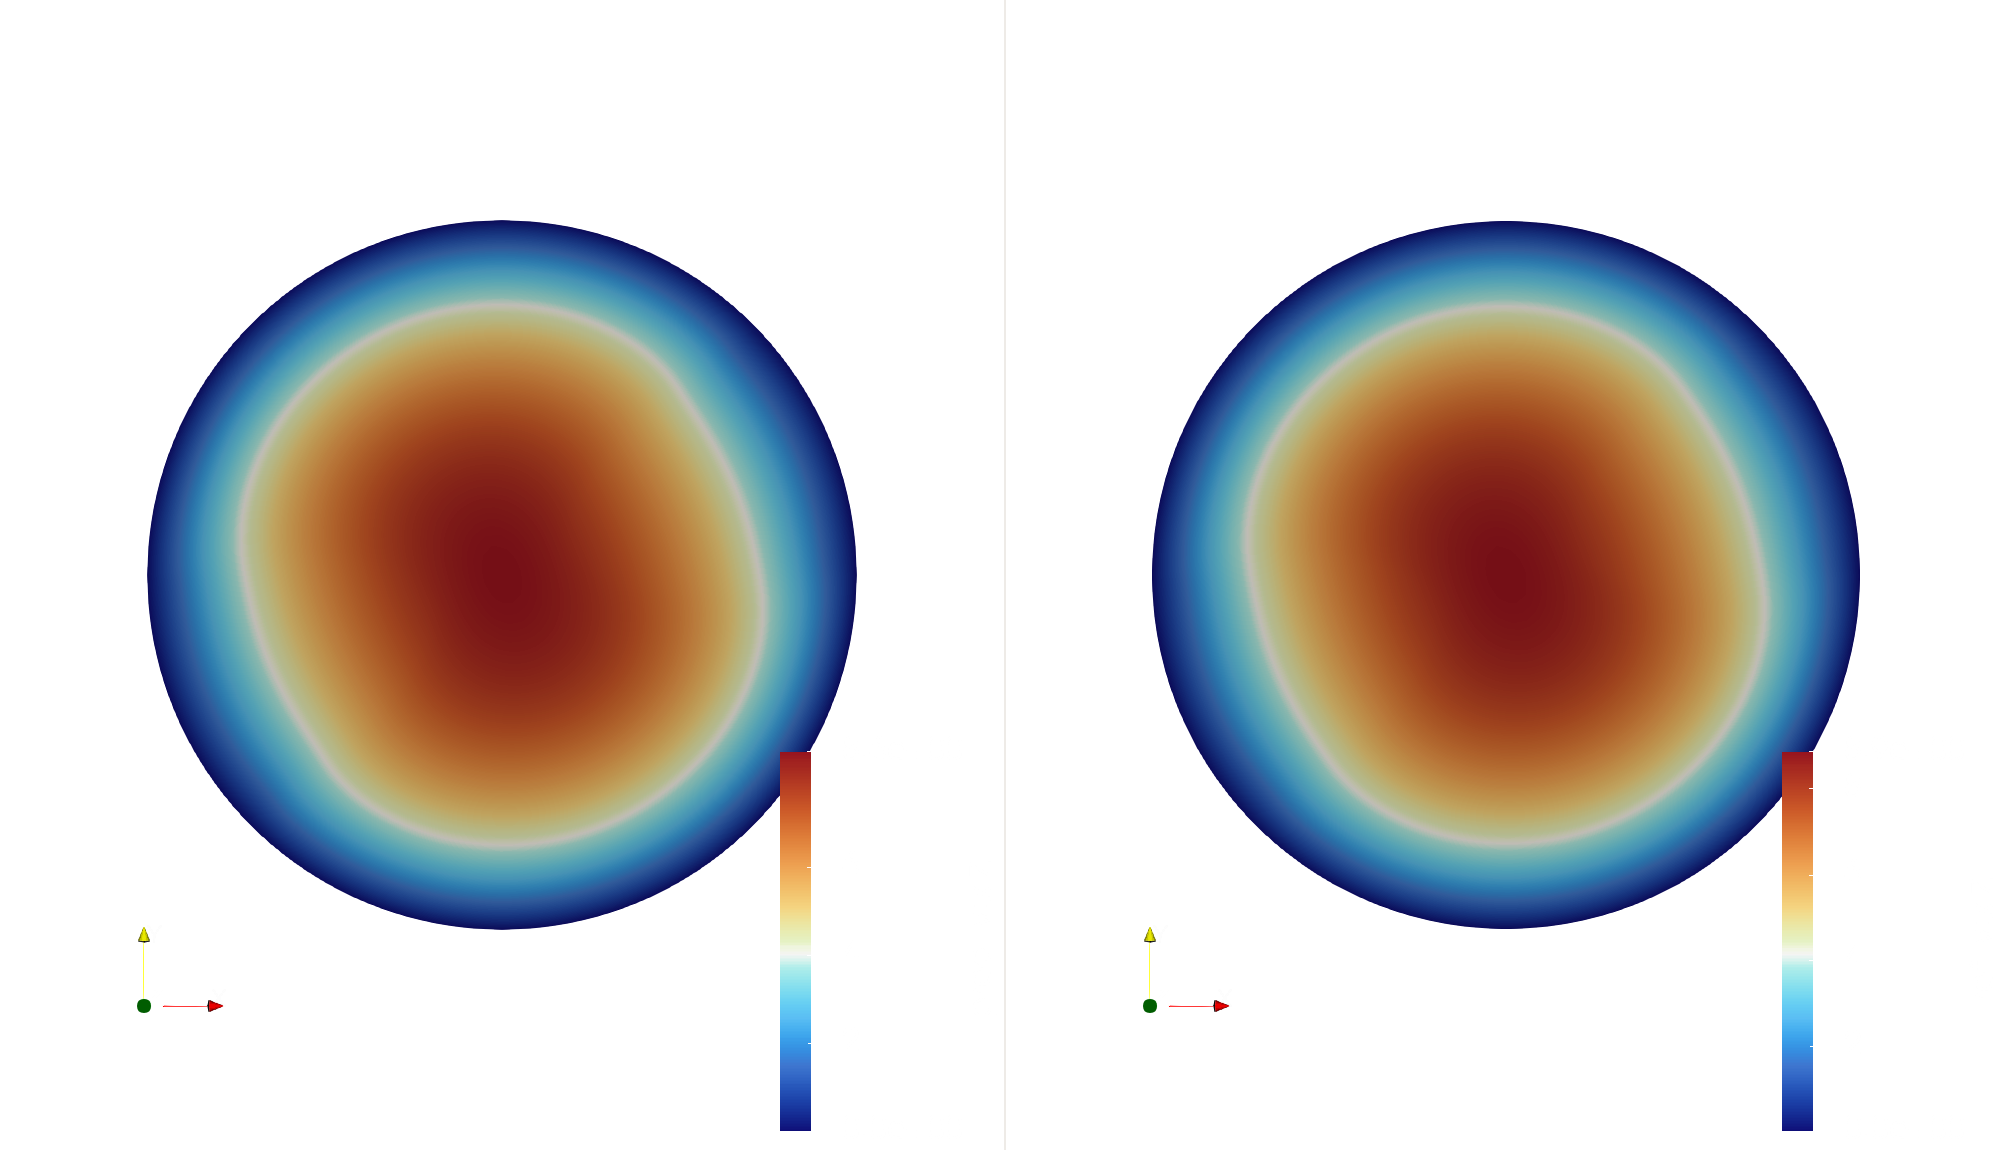
\includegraphics[width=0.8\textwidth]{img/bx_inf_u.png}
% \caption{Результаты численного эксперимента: поле деформаций при различных типах нагружения. Показаны компоненты деформации $u_{11}$, $u_{22}$ и $u_{12}$ для различных конфигураций нагружения.}
% \label{fig:numerical_deformations}
% \end{figure}

% \begin{figure}[htbp]
% \centering
% 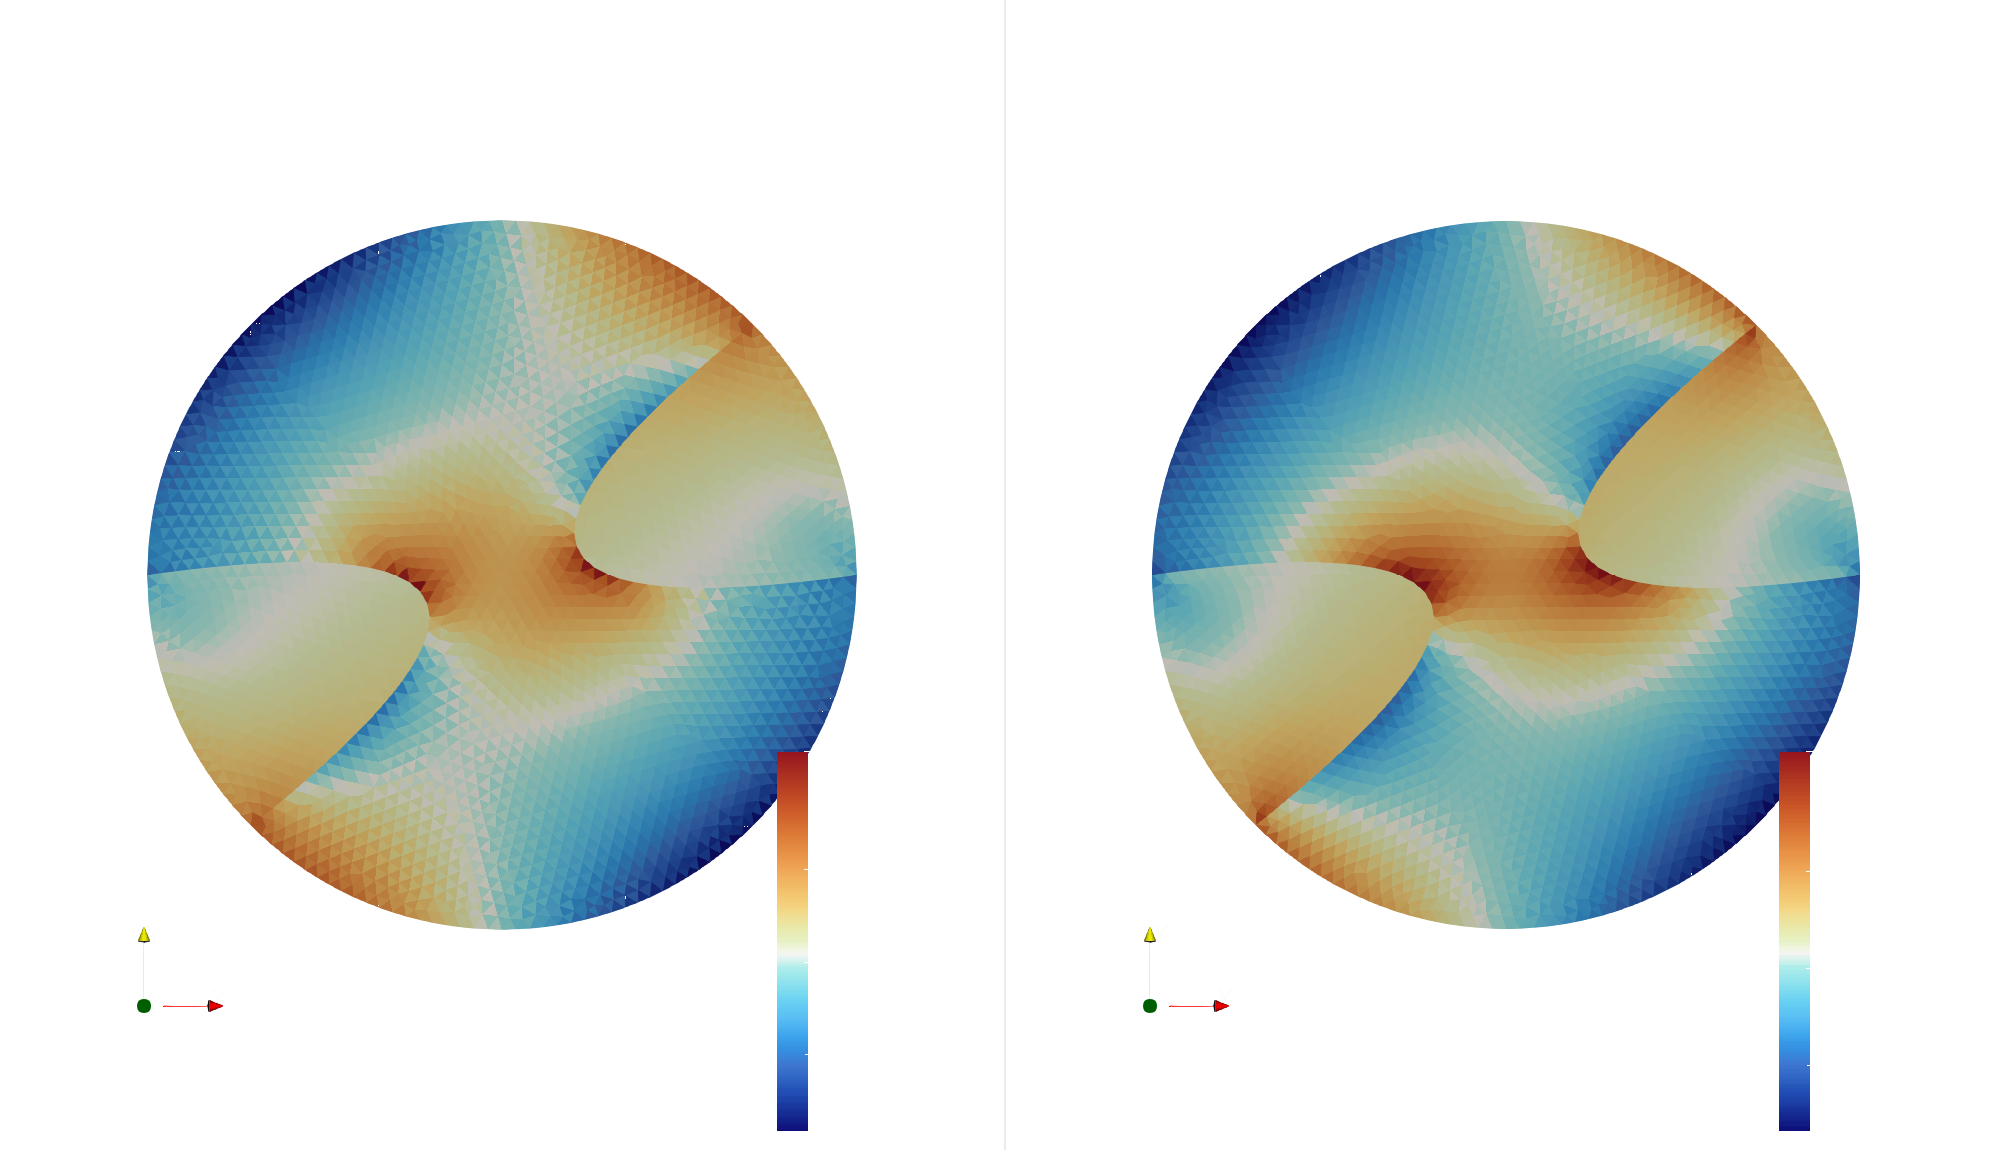
\includegraphics[width=0.8\textwidth]{img/bx_inf_S.png}
% \caption{Результаты численного эксперимента: поле напряжений ПК2. Показаны компоненты напряжений $S_{11}$, $S_{22}$ и $S_{12}$, вычисленные моделью CLANN для соответствующих деформаций.}
% \label{fig:numerical_stresses}
% \end{figure}

% \begin{figure}[htbp]
% \centering
% 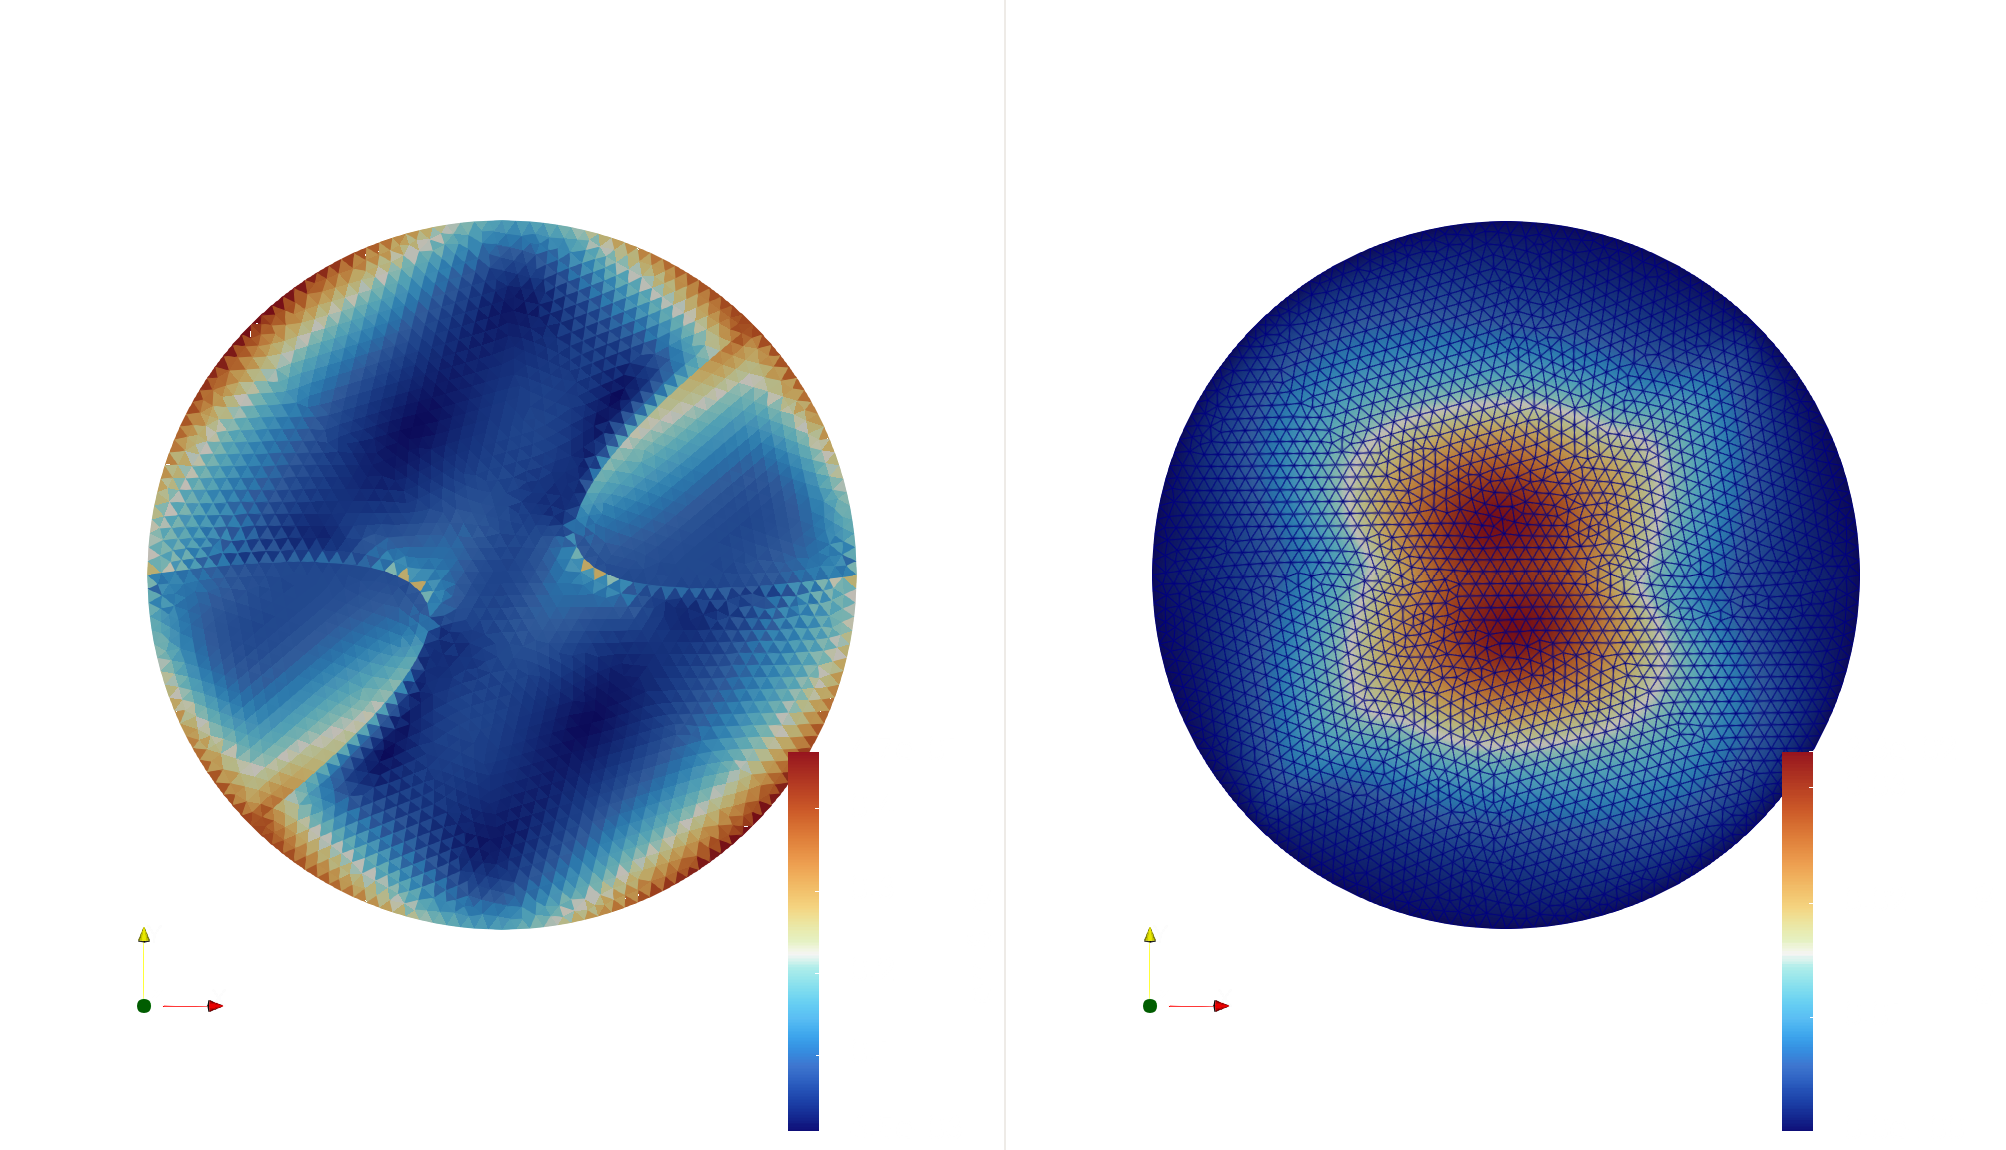
\includegraphics[width=0.8\textwidth]{img/bx_inf_err.png}
% \caption{Анализ ошибок численного эксперимента: распределение относительных ошибок между предсказанными и эталонными значениями напряжений. Показаны локальные и глобальные метрики точности модели.}
% \label{fig:numerical_errors}
% \end{figure}


% \section{Натурные эксперименты}
% % Здесь будет содержание натурных экспериментов
% \subsection{Экспериментальная установка}
% % Описание экспериментальной установки

% \subsection{Результаты и валидация}
% % Результаты натурных экспериментов

\section{Заключение}
% Здесь будет заключение


% \section{Математические и термодинамические свойства}
% \subsection{Выпуклость и устойчивость}
% Строгая выпуклость \(\psi\) обеспечивает единственность минимума, положительную определённость касательной жёсткости и устойчивость численного решения.

% \subsection{Развёрнутый вывод через цепное правило и эквивалентные формы}
% Полная потенциальная энергия деформации задаётся композиционно
% \begin{equation}
%  \Psi(\vect C) = \psi\big(\xi(\vect C)\big),\quad \vect C = \vect F^{\top} \vect F,\quad \vect C = \vect U^{\top} \vect U,\ \xi = (\ln u_{11},\,\ln u_{22},\, u_{12}/u_{11}).
% \end{equation}
% Тензор ПК2 определяется как
% \begin{equation}
%  \vect S = \frac{\partial \Psi}{\partial \vect C}.
% \end{equation}
% Применяя цепное правило к \(\Psi(\vect C)\), получаем эквивалентную запись
% \begin{equation}
%  \frac{\partial \Psi}{\partial \vect C} = \frac{\partial \psi}{\partial \xi} : \frac{\partial \xi}{\partial \vect C} \equiv \vect g(\xi) : \vect J(\vect C),
% \end{equation}
% где \(\vect g(\xi)=\partial\psi/\partial\xi\in\mathbb{R}^3\) и \(\vect J(\vect C)=\partial\xi/\partial \vect C\) — тензор Якоби. В размерности 2D при выбранной параметризации и разложении Холецкого \(\vect C=\vect U^{\top} \vect U\) аналитическая подстановка даёт явные формулы для компонент \(\vect S\).

\appendix

\chapter{\texorpdfstring{Эквивалентность QR-факторизации $\vect F$ и разложения Холецкого $\vect C=\vect F^{\top}\vect F$ для вычисления логарифмических координат $\boldsymbol{\xi}$}{Эквивалентность QR и Холецкого}}
\label{app:cholesky}

\section{Постановка и обозначения}

Рассматривается двумерная гиперупругая кинематика. Пусть:
\begin{itemize}
  \item $\vect F \in \mathbb{R}^{2 \times 2}$ — градиент деформации, $\det \vect F > 0$,
  \item $\vect C = \vect F^{\top}\vect F$ — правый тензор Коши–Грина (симметричный положительно определённый, SPD),
  \item Холецкий: $\vect C = \vect U^{\top}\vect U$, где $\vect U$ — верхнетреугольная и $\text{diag}(\vect U) > 0$,
  \item Логарифмические координаты:
    $\boldsymbol{\xi} = (\xi_1, \xi_2, \xi_3) = (\ln u_{11}, \ln u_{22}, u_{12}/u_{11})$.
\end{itemize}

Цель: показать, что при наличии $\vect F$ можно заменить вычисление $\vect U = \text{chol}(\vect C)$ на $\vect U = \vect R$ из тонкого QR($\vect F$) = $\vect Q \vect R$ (с $\text{diag}(\vect R) > 0$), и получить те же $\boldsymbol{\xi}$.

\section{Теорема (эквивалентность U и R)}

Пусть $\vect F \in \mathbb{R}^{2 \times 2}$ невырождённая ($\det \vect F > 0$). Рассмотрим тонкую QR-факторизацию
\begin{equation}
\vect F = \vect Q \vect R,
\end{equation}
где $\vect Q \in \mathbb{R}^{2 \times 2}$ — ортогональная ($\vect Q^{\top}\vect Q = \vect I$), $\vect R \in \mathbb{R}^{2 \times 2}$ — верхнетреугольная. Выберем стандартную нормализацию $\text{diag}(\vect R) > 0$. Тогда $\vect R$ совпадает с фактором Холецкого для $\vect C$:
\begin{equation}
\vect R = \text{chol}(\vect C), \quad \text{с} \quad \vect C = \vect F^{\top}\vect F.
\end{equation}

\textbf{Доказательство.}
\begin{equation}
\vect C = \vect F^{\top}\vect F = (\vect Q \vect R)^{\top}(\vect Q \vect R) = \vect R^{\top} \vect Q^{\top} \vect Q \vect R = \vect R^{\top} \vect R.
\end{equation}
Так как $\vect C$ — SPD и $\vect R$ — верхнетреугольная с положительной диагональю, то представление $\vect C = \vect R^{\top}\vect R$ единственно. По единственности фактора Холецкого (с $\text{diag} > 0$) следует $\vect R = \text{chol}(\vect C)$. $\square$

\textbf{Следствие.} Логарифмические координаты $\boldsymbol{\xi}$, определённые через $\vect U = \text{chol}(\vect C)$, можно эквивалентно вычислять из $\vect U = \vect R$ в QR($\vect F$), при условии $\text{diag}(\vect R) > 0$.

\section{Координаты $\vect{\xi}$ через $\vect{U}$}

Для $\vect U = \begin{bmatrix} u_{11} & u_{12} \\ 0 & u_{22} \end{bmatrix}$, $\text{diag}(\vect U) > 0$,
\begin{equation}
\boldsymbol{\xi} = (\xi_1, \xi_2, \xi_3) = (\ln u_{11}, \ln u_{22}, u_{12}/u_{11}).
\end{equation}
Тем самым, $\boldsymbol{\xi}(\vect F) := \boldsymbol{\xi}(\vect R(\vect F)) = \boldsymbol{\xi}(\vect U(\vect C))$.


